% Standalone build of the revision-4 material (to check it compiles and to review it on its own).
% In the paper, \input the individual files at the places named in their headers instead.
\documentclass[conference]{IEEEtran}
\usepackage{amsmath,amssymb,amsthm,graphicx,booktabs,algorithm,algpseudocode,hyperref}
\newtheorem{proposition}{Proposition}
\newcommand{\valCells}{18}
\newcommand{\valAgree}{15}
\newcommand{\valRhoTime}{0.93}
\newcommand{\valRhoLoss}{0.86}
\newcommand{\valMAE}{5.7}
\newcommand{\valPoints}{54}

\newcommand{\simRunsUDP}{11{,}520}
\newcommand{\simRunsTCP}{11{,}520}
\newcommand{\simRunsEcmp}{3{,}360}
\newcommand{\simSeeds}{30}

\IfFileExists{generated/sweep_macros.tex}{\newcommand{\sweepN}{1{,}945}
\newcommand{\sweepRuns}{13{,}615}
\newcommand{\sweepDefend}{61}
\newcommand{\sweepTopos}{10}
\newcommand{\sweepGapstatic}{1.00}
\newcommand{\sweepGapmpksp}{0.49}
\newcommand{\sweepGapsimplereactive}{1.44}
\newcommand{\sweepGaptelpexcess}{0.09}
\newcommand{\sweepGapresilientsdn}{0.70}
\newcommand{\sweepGapresilientsdnvTwo}{0.52}
\newcommand{\sweepGapresilientsdnvThree}{0.40}
}{}
\IfFileExists{generated/floor_macros.tex}{\newcommand{\floorMaxRel}{56.4}
\newcommand{\floorMedRel}{0.0}
\newcommand{\floorCells}{20}
\newcommand{\floorFlips}{6}
}{}
\begin{document}
\title{ResilientSDN -- Revision 4 Material}
\author{\IEEEauthorblockN{(authors as in the paper)}}
\maketitle

\section{Model}
% In the paper the score is Eq. (score) of Sec. III-D; repeated here so the file is self-contained.
For a candidate path $q$ of flow $f$:
\begin{equation}
 \mathrm{Score}(q)=w_1C(q)+w_2L(q)-w_3K_f(q).\label{eq:score}
\end{equation}
% Revision 4 -- notation for Sec. III-C. Replace the paper's notation table, or add the rows it lacks.
\begin{table}[t]\centering\footnotesize
\caption{Notation}\label{tab:notation}
\begin{tabular}{@{}ll@{}}
\toprule
Symbol & Meaning \\
\midrule
$G=(V,E)$, $c_e$ & directed network, capacity of link $e$ (bytes/s) \\
$t$, $\tau$ & polling interval index, its length (2\,s) \\
$\mathcal{F}(t)=\mathcal{F}_L\cup\mathcal{F}_A$ & flows (legitimate $\cup$ attack; not distinguishable) \\
$s_f,d_f,r_f(t)$ & ingress, egress switch and measured rate of flow $f$ \\
$\mathcal{A}$, $B_a$, $\mathcal{F}_a$ & attackers, rate budget and flows of attacker $a$ \\
$T_a(t)$, $T(t)$ & target links of attacker $a$; all targets \\
$\pi_a$, $\Delta_a$ & attacker's re-targeting policy and observation delay \\
$\mathcal{P}_f^H$ & simple paths of $f$ with at most $H$ hops \\
$x_f^p(t)$ & 1 if $f$ uses path $p$ in interval $t$ \\
$y_e$, $u_e$, $\hat u_e$ & load, utilisation, measured utilisation $\min\{1,u_e\}$ \\
$\theta$ & congestion threshold (0.8) \\
$\phi_e$, $\Phi$ & excess $[u_e-\theta]^+$ of a link; of the network \\
$\ell_f$, $K_f$ & path latency; normalised reconfiguration cost \\
$\beta,\gamma$ & weights of latency and reconfiguration in (\ref{eq:objective}) \\
$T_c$, $t_f^{\mathrm{last}}$ & cooldown; interval of $f$'s last move \\
$Q_e$, $V_0$, $\varepsilon$ & virtual queue, DPP penalty weight, deadband \\
$N$, $W$ & polls above $\theta$ to trigger; repeat-attack window \\
$w_1,w_2,w_3$ & score weights of $C$, $L$, $K$ (Eq.~\ref{eq:score}) \\
$U$, $s_e$ & max.\ utilisation (TE-LP); excess slack (TE-$\Phi$) \\
\bottomrule
\end{tabular}
\end{table}

% Revision 4 -- drop-in replacement for Section III-C (Problem Formulation) and Eq. (3).
% Notation table entries referenced here: Table~\ref{tab:notation}.
\subsection{Problem Formulation}\label{sec:formulation}

\paragraph{Network and traffic}
The data plane is a directed graph $G=(V,E)$; every full-duplex cable gives two directed links
$e=(i,j)$ with capacity $c_e$ (bytes/s). Time is divided into polling intervals
$t=1,2,\dots$ of length $\tau$ ($\tau=2$\,s). In interval $t$ the controller sees a set of flows
$\mathcal{F}(t)$, one per source--destination address pair (the granularity of the installed
OpenFlow rules). Flow $f$ enters at switch $s_f$, leaves at $d_f$ and offers rate $r_f(t)$,
measured at its ingress switch; $\mathbf{r}(t)=(r_f(t))_f$ is the traffic demand of interval $t$.
$\mathcal{F}(t)=\mathcal{F}_L(t)\cup\mathcal{F}_A(t)$ is the union of legitimate and attack
flows, but the controller cannot tell them apart: attack flows of a link-flooding attack are
individually low-rate and protocol-conformant~\cite{kang2013crossfire}, so the formulation never
uses the partition.

\paragraph{Attackers}
A set $\mathcal{A}$ of attackers; attacker $a$ controls bots that open flows
$\mathcal{F}_a(t)\subseteq\mathcal{F}_A(t)$ under a rate budget $\sum_{f\in\mathcal{F}_a(t)}
r_f(t)\le B_a$. Attacker $a$ aims at a set of target links $T_a(t)\subseteq E$; the attacked
set is $T(t)=\bigcup_a T_a(t)$, so $|T(t)|>1$ covers simultaneous multi-link attacks. An attacker
is \emph{adaptive} if it re-chooses its targets from the routes it observes,
$T_a(t)=\pi_a\big(\mathbf{x}(t-\Delta_a)\big)$, with an observation delay $\Delta_a$
(e.g.\ traceroute, as in Crossfire's rolling attack~\cite{kang2013crossfire}). Scenarios
S2--S11 are the case $|\mathcal{A}|=1$, $|T|=1$, $\pi_a$ constant; S12/S13 have $|T|=2,3$; S14
is adaptive (Sec.~\ref{sec:scenarios}).

\paragraph{Routing}
$\mathcal{P}_f^H$ is the set of simple $s_f$--$d_f$ paths with at most $H$ hops. The routing
decision is $x_f^p(t)\in\{0,1\}$ with $\sum_{p\in\mathcal{P}_f^H}x_f^p(t)=1$: every flow uses
exactly one path, because a flow is one exact-match rule per switch (splitting one address pair
needs select groups and per-packet hashing, which ResilientSDN does not use). The load and
utilisation of link $e$ are
\begin{equation}
  y_e(t)=\sum_{f\in\mathcal{F}(t)}\sum_{p\ni e} r_f(t)\,x_f^p(t),\qquad
  u_e(t)=\frac{y_e(t)}{c_e}.
  \label{eq:load}
\end{equation}
OpenFlow port counters report carried, not offered, bytes, so the controller observes
$\hat u_e(t)=\min\{1,u_e(t)\}$: an overloaded link reads as $100\,\%$ whatever its overload.

\paragraph{Objective}
With a congestion threshold $\theta\in(0,1)$ ($\theta=0.8$), the excess of link $e$ is
$\phi_e(t)=[u_e(t)-\theta]^+$ and the excess of the network is
$\Phi(\mathbf{x}(t))=\sum_{e\in E}\phi_e(t)$; $\Phi=0$ means that no link, attacked or not, is
above the threshold. Moving flow $f$ from path $p$ to $q$ installs a rule on every switch of $q$
that is not on $p$; the normalised reconfiguration cost is
$K_f(\mathbf{x}(t),\mathbf{x}(t-1))=|q\setminus p|/|q|$ (0 if $f$ stays), and $\ell_f$ is the
propagation latency of $f$'s path. The ideal controller solves, over a horizon of $\mathcal{T}$
intervals,
\begin{align}
  \min_{\mathbf{x}(1),\dots,\mathbf{x}(\mathcal{T})}\;
   & \frac{1}{\mathcal{T}}\sum_{t=1}^{\mathcal{T}}\Big[\Phi(\mathbf{x}(t))
     + \beta\sum_{f}\ell_f(\mathbf{x}(t))
     + \gamma\sum_{f}K_f(\mathbf{x}(t),\mathbf{x}(t-1))\Big]
     \label{eq:objective}\\
  \text{s.t.}\;
   & \textstyle\sum_{p\in\mathcal{P}_f^H}x_f^p(t)=1,\quad x_f^p(t)\in\{0,1\}
     && \forall f,t \label{eq:unsplit}\\
   & x_f(t)\neq x_f(t-1)\;\Rightarrow\; t-t_f^{\mathrm{last}}\ge T_c/\tau
     && \forall f,t \label{eq:cooldown}
\end{align}
where $t_f^{\mathrm{last}}$ is the interval of $f$'s previous move and $T_c$ the cooldown.
Eq.~(\ref{eq:objective}) replaces the single-link objective of the earlier version (old Eq.~3):
it covers any number of attackers and target links, any demand $\mathbf{r}(t)$ (attack flows
included) and any topology through $G$, $c_e$ and $\mathcal{P}_f^H$; and it charges congestion
created on \emph{non-attacked} links (secondary congestion) exactly as congestion on a target.

\paragraph{Hardness and the relaxation used as a baseline}
For a single interval with $\beta=\gamma=0$, deciding whether $\Phi=0$ is feasible is the
decision version of unsplittable minimum-congestion routing, which is NP-hard already for a single
source~\cite{kleinberg1996unsplittable}. Relaxing (\ref{eq:unsplit}) to $x_f^p\in[0,1]$ and
minimising the maximum utilisation $U$ instead of $\Phi$ gives the path-flow linear program
\begin{equation}
  \min U\quad\text{s.t.}\quad
  \sum_{f}\sum_{p\ni e} r_f\,x_f^p\le U c_e\;\forall e,\qquad
  \sum_{p}x_f^p=1,\; x_f^p\ge 0\;\forall f,
  \label{eq:lp}
\end{equation}
the classical min-max-utilisation TE problem; replacing $U$ by $\sum_e s_e$ with
$s_e\ge u_e-\theta$ gives the LP relaxation of (\ref{eq:objective}) itself (TE-$\Phi$). Its optimum $U^\star$ is a lower bound on the
maximum utilisation of every routing, split or not, over the same path sets and the same measured
demand. We implement both as baselines (TE-LP and TE-$\Phi$, Sec.~\ref{sec:baselines}); the gap between
ResilientSDN and them measures the cost of single-path, rule-economical operation. Min-max is
degenerate when some link is overloaded whatever the routing, which the excess objective is not.

\paragraph{Instance optimum and defendability}
Path-based relaxations are lower bounds only for the path sets they use. To compare every system
with the best \emph{any} controller could do on the same traffic, we solve the arc-based
multicommodity relaxation of (\ref{eq:objective}) with $\beta=\gamma=0$ in each interval,
\begin{equation}
  \Phi^\star(t)=\min_{g\ge0,\,s\ge0}\;\sum_{e\in E}s_e\quad\text{s.t.}\quad
  \frac{1}{c_e}\sum_{k}g_{k,e}-s_e\le\theta\;\;\forall e,\qquad
  g_k\ \text{a flow of the demands of source }k,
  \label{eq:phistar}
\end{equation}
with commodities aggregated by source node (exact here, since $\Phi$ depends only on the total load per
link). Every routing of the same demand --- any paths, any hop count, split or not --- is feasible for
(\ref{eq:phistar}), so $\Phi^\star(t)\le\Phi(\mathbf{x}(t))$ for every controller, and
$\Phi^\star=\int\Phi^\star(t)\,dt$ bounds the excess any controller can achieve over an attack. We
call an instance \emph{defendable} if $\Phi^\star=0$, and measure a system by its
\emph{remaining excess} $(\Phi-\Phi^\star)/(\Phi_{\mathrm{static}}-\Phi^\star)$: 0 means optimal, 1
means no better than not reacting at all. The ideal latency- and reconfiguration-free controller of
(\ref{eq:objective}) is therefore not a hypothetical object: its value is computed for every evaluated
instance (Sec.~\ref{sec:sweep}).

\paragraph{When does the attacker win?}
Defendability is a property of the instance, not of the controller, and it has a simple necessary
condition. For a partition $(X,Y)$ of $V$, let $L(X,Y)$ be the links from $X$ to $Y$, $c(L)$ their
capacity and $D_{XY}$ the total demand (legitimate and attack) from sources in $X$ to destinations in
$Y$.
\begin{proposition}[cut condition]\label{prop:cut}
For every routing, split or not,
$\displaystyle \Phi\;\ge\;\frac{D_{XY}-\theta\,c(L)}{\max_{e\in L}c_e}$.
In particular no controller can keep every link at or below $\theta$ if some cut carries more than
$\theta$ times its capacity, and an attacker that can place bots on the $X$ side of a cut separating
them from destinations on the $Y$ side wins against every defence with a budget
$B>\theta\,c(L)-D^{L}_{XY}$, where $D^{L}_{XY}$ is the legitimate demand across the cut.
\end{proposition}
\begin{proof}
Every unit of demand from $X$ to $Y$ crosses $L(X,Y)$ at least once, so $\sum_{e\in L}y_e\ge D_{XY}$.
Hence $\sum_{e\in L}(u_e-\theta)c_e\ge D_{XY}-\theta c(L)$, and the left side is at most
$\max_{e\in L}c_e\sum_{e\in L}[u_e-\theta]^+\le\max_{e\in L}c_e\,\Phi$.
\end{proof}
This formalises the observation behind Crossfire~\cite{kang2013crossfire}: a link-flooding attacker
needs to beat the \emph{cut}, not a link, and rerouting can only help while the cut has spare capacity.
Proposition~\ref{prop:cut} is weaker than (\ref{eq:phistar}) (which takes every cut into account at
once) but explains the trend the sweep shows: the share of defendable instances falls as the attack
intensity and the number of attacked links grow.

\paragraph{The scenario space}
An evaluation instance is a point $\omega=(G,c,\mathbf{r}^L,\mathcal{A},\{B_a,T_a,\pi_a\})$ of the
model above: a topology with capacities, a legitimate demand matrix, and per attacker a budget, a target
set and a behaviour $\pi_a$ (constant, pulsing with period $P$ and duty $\delta$, timed bursts, or
rolling re-targeting). The scenarios S1--S14 are fourteen hand-chosen points of this space
(Table~\ref{tab:scenario_space}); the randomised sweep of Sec.~\ref{sec:sweep} samples it, so that the
conclusions are tested over the space rather than at a few points.

\paragraph{Online, myopic approximation}
The controller knows neither future demand nor the attacker's policy $\pi_a$, so it cannot solve
(\ref{eq:objective}) over the horizon. Following Lyapunov drift-plus-penalty
control~\cite{neely2010stochastic}, define for every link a virtual queue
$Q_e(t+1)=[Q_e(t)+y_e(t)-\theta c_e]^+$, which grows exactly while $e$ is above the threshold.
Minimising, in each interval, a bound on the drift $\mathbb{E}[\Delta Q]$ plus $V$ times the
penalty (reconfiguration) keeps the time-average excess bounded while trading it against rule
changes. ResilientSDN uses this structure with two approximations that the evaluation tests
explicitly: (i) the backlog weight of each link is replaced by its post-move utilisation, giving
the per-flow score
\begin{equation}
  \mathrm{DPP}(p)=-\sum_{e\in p}u_e^{\mathrm{post}}-V_0\,K_f(p),
  \label{eq:dpp}
\end{equation}
or, in the bottleneck variant, $-\max_{e\in p}u_e^{\mathrm{post}}-V_0K_f(p)$;
and (ii) flows are decided one at a time, greedily, with the loads updated after every move
(Algorithm~\ref{alg:rsdn}). A move is made only if it improves (\ref{eq:dpp}) by more than a
deadband $\varepsilon$, which together with (\ref{eq:cooldown}) is the stability mechanism.
The sum form penalises path length, so in sparse WANs it can hold a flow on a congested one-hop
link rather than move it to a long detour (observed on Internet2, Sec.~\ref{sec:results}); the
bottleneck form removes this bias.

\paragraph{What the greedy step guarantees}
Let the capacity filter admit $q$ for flow $f$ on congested link $e$ only if
$u_{e'}^{\mathrm{post}}\le\theta$ for every $e'\in q$, evaluated on the projected loads that
already include the moves made earlier in the same interval.
\begin{proposition}\label{prop:monotone}
With exact rates, every move accepted through the capacity filter strictly decreases $\Phi$, and
creates no new link above $\theta$. Hence within one interval Algorithm~\ref{alg:rsdn} performs at
most $|\mathcal{F}(t)|$ moves and never causes secondary congestion.
\end{proposition}
\begin{proof}
Removing $r_f>0$ from the old path $p\ni e$ lowers $y_{e'}$ for all $e'\in p$, so no $\phi_{e'}$
grows and $\phi_e$ falls by $\min(r_f,\,y_e-\theta c_e)/c_e>0$ because $e$ is above $\theta$.
Adding $r_f$ to $q$ leaves every $e'\in q$ at $u_{e'}\le\theta$, so $\phi_{e'}=0$ before and
after (links on both $p$ and $q$ carry $f$ before and after). Each flow is moved at most once
per interval (the cooldown), which bounds the number of moves.
\end{proof}
The guarantee is with respect to the \emph{measured} rates: if an attacker raises its rate in
the next interval (S8) or the measurement of an overloaded link is clipped at $\hat u_e=1$, the
projected and real loads differ, which is why secondary congestion is still measured. The optional
fallback (Algorithm~\ref{alg:rsdn}, line~\ref{alg:fallback}) gives up the second half of the
proposition: it accepts a path above $\theta$ whose bottleneck is still below $u_e$, so it never
raises the maximum utilisation when $e$ is the most loaded link (guaranteed by processing links in
decreasing utilisation), but may raise $\Phi$ on other links.

\paragraph{Bounded churn}
The cooldown makes the stability constraint (\ref{eq:cooldown}) hold by construction, which bounds the
disruption any traffic pattern can cause.
\begin{proposition}\label{prop:churn}
With cooldown $T_c>0$ (or cooldowns drawn from $[T_{\min},T_{\max}]$, $T_{\min}>0$, as in S10), during
any period of length $D$ each flow is moved at most $\lfloor D/T_c\rfloor+1$ times (resp.\
$\lfloor D/T_{\min}\rfloor+1$), and returns to a path it used before at most $\lfloor D/T_c\rfloor$ times.
\end{proposition}
\begin{proof}
Consecutive moves of the same flow are at least $T_c$ apart (Algorithm~\ref{alg:rsdn}, deadband and
cooldown line), so at most $\lfloor D/T_c\rfloor+1$ move instants fit in $D$; a return to an earlier path
is a move other than the first.
\end{proof}
With $T_c=30$\,s a flow moves at most 3 times in a 60\,s attack and 21 times in S6 (600\,s), whatever the
attacker does; ResilientSDN made 2.3 moves per run in total. Threshold-reactive rerouting has no such
bound: a flow can be moved at every poll ($D/\tau$ times), and it made 388 moves per run, 379 of them
back to an earlier path (Sec.~\ref{sec:results}).

\paragraph{How long can an attacker stay undetected?}
Call a poll \emph{hot} if $\hat u_e>\theta$. The trend detector fires on $N$ consecutive hot polls; the
optional duty-cycle rule (\textsc{DutyCycle} in Algorithm~\ref{alg:rsdn}) also fires on a hot poll when
at least $\lceil\rho M\rceil$ of the last $M$ polls were hot.
\begin{proposition}\label{prop:evasion}
Let $N$ be fixed. If the detector never fires on link $e$, then among any $n$ consecutive polls at most
$(N-1)\lceil n/N\rceil$ are hot (trend detector alone); with the duty-cycle rule, among any $n$
consecutive polls after the first $M-1$ at most $(\lceil\rho M\rceil-1)\lceil n/M\rceil$ are hot. The
bounds are attained when $n$ is a multiple of $N$, resp.\ $M$. Asymptotically, an undetected attacker keeps $e$ above $\theta$ at most a fraction
$(N-1)/N$, resp.\ $\min\{(N-1)/N,\,(\lceil\rho M\rceil-1)/M\}$, of the time.
\end{proposition}
\begin{proof}
Without detection no run of hot polls reaches length $N$, so each of the $\lceil n/N\rceil$ blocks of at
most $N$ polls contains a non-hot poll. For the duty rule, take any $M$ consecutive polls (all after
the first $M-1$) with at least $\lceil\rho M\rceil$ hot ones and let $j$ be the last hot one. The $M$
polls ending at $j$ contain every hot poll of that window, since they all lie between its start and
$j$, so the rule fires at $j$. Hence each of the $\lceil n/M\rceil$ blocks of at most $M$ polls holds at
most $\lceil\rho M\rceil-1$ hot polls. Repeating $N-1$ hot polls and one cool poll, resp.\
$\lceil\rho M\rceil-1$ hot and $M-\lceil\rho M\rceil+1$ cool, attains the bounds; an exhaustive check over
all hot/cool sequences of 14 polls against the detector code confirms them
(\texttt{tests/test\_detector.py}).
\end{proof}
With $N=3$ an undetected attacker can keep a link above $\theta$ two thirds of the time; S7 (hot half of
the time) is one such pattern. With $M=6$, $\rho=0.5$ the bound falls to one third, so S7 is detected,
while legitimate bursts that are hot in at most 2 of 6 polls (ablation D) are not. The proposition is
about \emph{detection}; whether a detected link is then relieved depends on the capacity available for
detours. An attacker can also hold a link just below $\theta$ indefinitely, which by definition is not
congestion; lowering $\theta$ trades this against more reaction to legitimate load.

\paragraph{Complexity}
Per interval the detector is $O(|E|)$. For each congested link and each flow on it, the candidate
set is enumerated once ($|\mathcal{P}_f^H|$ paths of at most $H$ links) and scored, so the
decision step is $O\big(|D(t)|\cdot\max_e|\mathcal{F}_e|\cdot|\mathcal{P}^H|\cdot H\big)$;
$|\mathcal{P}^H|$ is small on the fat-tree and bounded by the hop limit $H$ on the WANs.

% Revision 4 -- Algorithm 1, aligned line by line with controller/decision.py
% (ResilientDecision.on_interval / _try_reroute). Needs \usepackage{algorithm,algpseudocode}.
\begin{algorithm}[t]
\caption{ResilientSDN, one polling interval $t$}\label{alg:rsdn}
\begin{algorithmic}[1]
\Require loads $\hat y_e$, $\hat u_e$; rates $r_f$; paths $p_f$
\Statex \hspace{\algorithmicindent}parameters $\theta,N,H,w_{1..3},V_0,\varepsilon,T_c$
\State $D\gets\{e:\hat u_e>\theta$ in the last $N_e$ polls$\}$ \Comment{trend detector}
\Statex \hspace{\algorithmicindent}($N_e=N-1$ if $e$ was attacked in the last $W$\,s, else $N$;
\Statex \hspace{\algorithmicindent}\textsc{DutyCycle}: also if $\hat u_e>\theta$ now and in $\ge\rho M$ of the last $M$ polls)
\State \textbf{if} $D=\emptyset$ \textbf{return}
\State $\tilde y\gets\hat y$ \Comment{projected loads}
\State \textbf{if} \textsc{OrderBySeverity}: sort $D$ by $\tilde y_e/c_e$, descending
\ForAll{$e\in D$}
  \State $x_e\gets\tilde y_e-\theta c_e$ \Comment{excess to shed}
  \ForAll{$f$ with $e\in p_f$, by $r_f$ descending}
    \State \textbf{if} $x_e\le 0$ \textbf{break}
    \State $\tilde y^{-f}\gets\tilde y$ with $r_f$ removed from $p_f$
    \State $A\gets\{q\in\mathcal{P}_f^H: e\notin q,\ q\neq p_f\}$
    \State $P\gets\{q\in A:\max_{e'\in q}(\tilde y^{-f}_{e'}+r_f)/c_{e'}\le\theta\}$
    \Statex \hfill\Comment{capacity filter}
    \If{$P=\emptyset$ \textbf{and} \textsc{Fallback}} \label{alg:fallback}
      \State $q^\circ\gets\arg\min_{q\in A}\max_{e'\in q}(\tilde y^{-f}_{e'}+r_f)/c_{e'}$
      \State \textbf{if} that value $<\tilde y_e/c_e$: $P\gets\{q^\circ\}$, relief $\gets$ true
    \EndIf
    \State \textbf{if} $P=\emptyset$: log \textit{no\_candidate}; \textbf{continue}
    \State $q^\star\gets\arg\max_{q\in P}\mathrm{Score}(q)$ \Comment{Eq.~(\ref{eq:score})}
    \State $\delta\gets\mathrm{DPP}(q^\star;\tilde y^{-f})-\mathrm{DPP}(p_f;\tilde y)$
      \Comment{Eq.~(\ref{eq:dpp})}
    \If{($\delta\le\varepsilon$ \textbf{and not} relief) \textbf{or} $t-t_f^{\mathrm{last}}<T_c$}
      \State log \textit{held}; \textbf{continue} \Comment{deadband and cooldown}
    \EndIf
    \State install $q^\star$ make-before-break; $t_f^{\mathrm{last}}\gets t$
    \State $\tilde y\gets\tilde y^{-f}$ with $r_f$ added on $q^\star$;\quad $x_e\gets x_e-r_f$
  \EndFor
  \State \textbf{if} $x_e>0$: log \textit{unresolved}$(e,x_e)$
\EndFor
\end{algorithmic}
\end{algorithm}
% Published configuration: OrderBySeverity = Fallback = false, sum drift, V0 = 1.
% ResilientSDN-v2 (revision 4, simulation): OrderBySeverity = Fallback = true,
% bottleneck drift with V0 = 0.1. ResilientSDN-v3: v2 + DutyCycle (M = 6, rho = 0.5). C(q) = 1 - max post-move utilisation, L(q) = best candidate
% latency / latency(q), K_f(q) = |q \ p_f| / |q|  (controller/scorer.py).


\section{Evaluation additions}
% Revision 4 -- additions to Section IV/V (evaluation setup). Insert after the existing scenario
% table; the S1-S11 definitions are unchanged.

\subsection{Additional attack scenarios}\label{sec:scenarios}
Three scenarios exercise the generalised model of Sec.~\ref{sec:formulation}:
\begin{itemize}
\item \textbf{S12 / S13, multi-link.} Two (S12) or three (S13) target links are attacked at
  once, each by 3 flows of 30\,Mbps (the S11 overload, per link) for 120\,s, with two legitimate
  flows per target. Targets are the most-used fastest non-bridge links under static routing that
  share no switch with an earlier target.
\item \textbf{S14, adaptive rolling attacker.} The S11 budget (3 flows $\times$ 30\,Mbps, 120\,s),
  but every $\Delta_a=10$\,s the attacker observes the victims' current routes and re-aims at the
  link that most victim flows now share. It keeps flows that already cross that link and replaces
  the others with flows from fresh host pairs, chosen so that the \emph{defence's own} routing of a
  new flow (static, ECMP hash, $k$-path split, \dots) puts the largest share of the flow on the link.
  This is the rolling behaviour of Crossfire~\cite{kang2013crossfire} with a routing-aware
  attacker, i.e.\ the strongest attacker the threat model allows.
\end{itemize}
S12--S14 are evaluated in simulation only (Sec.~\ref{sec:sim}).
Table~\ref{tab:scenario_space} places every scenario in the scenario space of
Sec.~\ref{sec:formulation}, together with the ranges from which the randomised sweep of
Sec.~\ref{sec:sweep} draws 2{,}000 further instances.
% Revision 4 -- the hand-made scenarios as points of the scenario space (Sec. III-C), and the ranges the
% randomised sweep samples (sim/generic.py). alpha = target's offered load / capacity during the attack
% (legitimate 20 Mbps included), as in the measured-load checks of the emulation.
\begin{table}[t]\centering\scriptsize
\caption{Scenarios as points of the space $\omega=(G,c,\mathbf{r}^L,\mathcal{A},B_a,T_a,\pi_a)$ and the
ranges sampled by the randomised sweep.}\label{tab:scenario_space}
\setlength{\tabcolsep}{2.5pt}
\begin{tabular}{@{}lccccl@{}}
\toprule
 & topologies & $|T|$ & bots/target & $\alpha$ & behaviour $\pi_a$\\
\midrule
S1 & 4 & 0 & 0 & 0.2 & none\\
S2--S5 & 4 & 1 & 1--5 & 0.5--0.95 & constant\\
S6, S11 & 4 & 1 & 3 & 1.1 & constant, 600 / 120\,s\\
S7 & 4 & 1 & 3 & 0.85 / 0.65 & pulse, $P=8$\,s, $\delta=\tfrac12$\\
S8 & 4 & 1 & 3 & 0.9 & bursts of 8\,s every 31\,s\\
S9 & 4 & 1 & 3 & 0.9 & constant, detours pre-loaded to 0.79\\
S10 & 4 & 1 & 3 & as S7--S9 & S7--S9, randomised $N$, $T_c$\\
S12, S13 & 4 & 2, 3 & 3 & 1.1 & constant\\
S14 & 4 & 1 (moving) & 3 & 1.1 & rolling, $\Delta=10$\,s\\
SB & 4 & 0 & 0 & 0.9 in bursts & legitimate bursts only\\
\midrule
Sweep & 8 real + Waxman, BA & 1--3 & 1--5 & U[0.9, 1.6] & constant, pulse ($P\in\{4,8\}$,\\
 & (15--40 nodes) & & & & $\delta\in\{\tfrac13,\tfrac12,\tfrac23\}$), timed, rolling\\
 & \multicolumn{5}{l}{legitimate demand: gravity model, 10--60 flows, base load U[0.2, 0.6]}\\
\bottomrule
\end{tabular}
\end{table}


\subsection{Additional baselines}\label{sec:baselines}
Besides static shortest-path routing, static ECMP~\cite{rfc2992} and simple reactive rerouting, three
baselines represent multipath routing and optimal traffic engineering:
\begin{itemize}
\item \textbf{$k$-path multipath ($k$-MP)}: every flow is split equally over its $k=3$
  lowest-latency paths within the hop limit and never moved (oblivious, traffic-unaware spreading).
\item \textbf{TE-LP}: whenever any link is above $\theta$, the controller solves the min-max-utilisation
  LP~(\ref{eq:lp}) (HiGHS) over the $K=6$ lowest-latency paths of every active flow, with the
  measured rates of \emph{all} flows, and installs the fractional split. Ties are broken towards
  the current split and shorter paths so that equal-optimum solutions do not churn. It reacts on
  the first poll above $\theta$ (no trend detector) and splits single flows, which needs weighted
  select groups: it is an idealised TE upper bound in the spirit of
  SWAN/B4~\cite{hong2013swan,jain2013b4}, not a deployable equal of ResilientSDN.
\item \textbf{TE-$\Phi$}: the same LP with the objective of Eq.~(\ref{eq:objective}) instead of the
  maximum: minimise $\sum_e s_e$ with $s_e\ge u_e-\theta$, $s_e\ge0$ (the maximum utilisation only
  breaks ties), i.e.\ the LP relaxation of our own per-interval problem. We added it after observing
  that min-max TE is degenerate on G\'EANT: in 12 of 30 S11 runs a 5\,Mbps background flow on a
  1.55\,Mbps link (no detour among its candidate paths) fixes $U^\star=3.23$ whatever the routing, so
  every split that keeps the attacked link below 3.23 is optimal and the LP never relieves it.
\end{itemize}
\textbf{ResilientSDN-v2} is Algorithm~\ref{alg:rsdn} with the two extensions turned on (severity
order, fallback) and the bottleneck form of~(\ref{eq:dpp}) with $V_0=0.1$; ResilientSDN without
suffix is the published configuration. \textbf{ResilientSDN-v3} adds a duty-cycle trigger to v2: a
link that is above $\theta$ now also counts as congested if it was above $\theta$ in at least half of the
last $M=6$ polls (12\,s). It targets the pulse attack S7, which alternates 85\,\% and 65\,\% load every
4\,s and so is never above $\theta$ for $N=3$ consecutive polls; the legitimate bursts of ablation D
(above $\theta$ in at most 2 of 6 polls) must not trigger it, which we test with the scenario
\textbf{SB} (S1 traffic plus those bursts).

\subsection{Flow-level simulation}\label{sec:sim}
The Mininet testbed takes about 90\,s per run (630\,s for S6), which limits it to five runs per
cell and to the scenarios already reported. To add seeds, scenarios, TCP traffic and the LP baseline
we built a flow-level simulator (\texttt{sim/}) that runs the \emph{same decision code} as the Ryu
controller (Algorithm~\ref{alg:rsdn} lives in one module imported by both) and the same traffic
planner, so targets, host pairs and rates are identical to the emulation for the same seed.
The model advances in 1\,s steps:
UDP flows are inelastic and an overloaded link drops the excess in proportion to arriving rates
(with upstream drops propagated downstream);
TCP flows are elastic 5\,MB transfers (access cap 20\,Mbps, 1\,s think time between transfers) that
share what UDP leaves by max-min fairness~\cite{bertsekas1992data}, with a floor of 5\,\% of a
saturated link (TCP is not modelled as starving completely under drop-tail).
The controller sees what OpenFlow counters would report: carried link load ($\le c_e$) and the
ingress rate of every flow, averaged over the 2\,s polling interval. Not modelled: queueing delay,
TCP dynamics below the 1\,s step (slow start, reordering after a path change), packet-level
burstiness and control-plane latency.
\textbf{Validation.} On the \valCells\ (topology, scenario) cells and \valPoints\ (cell, system)
points that both the simulator and an earlier emulation campaign (1~October 2026, 390 runs, same
traffic protocol; its summary table is in \texttt{paper\_rev4/data}) cover, the Spearman correlation
of seconds above threshold is \valRhoTime\ (loss: \valRhoLoss), and the simulator ranks the three
systems the same way as the emulation in \valAgree\ of \valCells\ cells
(Fig.~\ref{fig:validation}). The main systematic difference is that the simulator relieves a link
about 2\,s earlier (no rule-installation delay). We therefore use the simulator for relative
comparisons across many seeds and scenarios, and the emulation for absolute values.

\begin{figure}[t]\centering
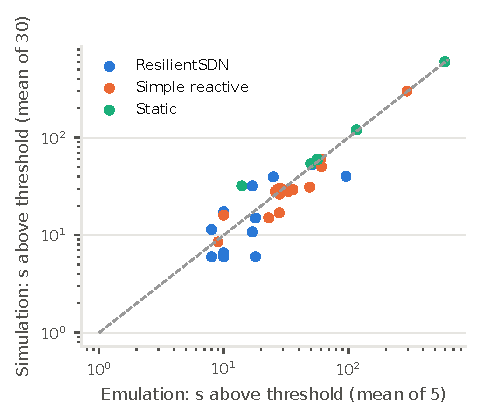
\includegraphics[width=\columnwidth]{figures/validation}
\caption{Simulation against emulation: mean seconds above $\theta$ per (topology, scenario, system).
Dashed: identity.}\label{fig:validation}
\end{figure}

\subsection{Seeds and statistics}\label{sec:stats}
Simulation cells use 30 seeds (\simRunsUDP\ UDP runs, \simRunsTCP\ TCP runs, \simRunsEcmp\ runs
with an ECMP-aware attacker); emulation cells keep 5. Run $r$ of a cell gives every system the same
traffic, so comparisons are \emph{paired}: for each cell, metric and system we report the mean
per-seed difference to ResilientSDN with a 95\,\% percentile-bootstrap CI (10\,000 resamples), the
two-sided Wilcoxon signed-rank test~\cite{wilcoxon1945}, the matched-pairs rank-biserial
correlation as effect size~\cite{kerby2014rankbiserial}, and Holm-Bonferroni
correction~\cite{holm1979} over all tests of a table. This replaces the earlier unpaired,
uncorrected Welch tests (\texttt{evaluation/paired\_stats.py}).

% Revision 4 -- new results subsections. Numbers in the text are from paper_rev4/generated/*.csv
% (make_assets.py); every table/figure is generated, none is typed by hand.
\subsection{Revision-4 results}\label{sec:results}

\begin{table*}[t]\centering\scriptsize
\caption{Simulation, UDP legitimate traffic: seconds with a target link above $\theta=0.8$ (mean $\pm$ 95\% CI over 30 seeds; lowest in bold).}\label{tab:sim_time}
\setlength{\tabcolsep}{3pt}
\begin{tabular}{llrrrrrrrr}
\toprule
Topology & Scen. & Static & ECMP & k-MP & Reactive & TE-LP & TE-$\Phi$ & RSDN & RSDN-v2\\
\midrule
Fat-tree & S3 & 60 & \textbf{0} & \textbf{0} & 28$\pm$3 & 2 & 2 & 6 & 6\\
 & S5 & 60 & \textbf{0} & \textbf{0} & 30 & 2 & 2 & 6 & 6\\
 & S6 & 600 & \textbf{0} & \textbf{0} & 300 & 2 & 2 & 6 & 6\\
 & S7 & 32 & \textbf{0} & \textbf{0} & 16 & 2 & 2 & 32 & 32\\
 & S8 & 14 & \textbf{0} & \textbf{0} & 8 & 2 & 2 & 6 & 6\\
 & S9 & 54 & \textbf{0} & \textbf{0} & 28 & 2 & 2 & 6 & 6\\
 & S10 & 33$\pm$6 & \textbf{0} & \textbf{0} & 17$\pm$3 & 2 & 2 & 8$\pm$1 & 8$\pm$1\\
 & S11 & 120 & \textbf{0} & \textbf{0} & 60 & 2 & 2 & 6 & 6\\
 & S12 & 120 & 20$\pm$17 & 48$\pm$22 & 62$\pm$4 & \textbf{6$\pm$8} & \textbf{6$\pm$8} & 12$\pm$8 & 8$\pm$1\\
 & S13 & 120 & 52$\pm$23 & 84$\pm$21 & 62$\pm$4 & \textbf{10$\pm$11} & 10$\pm$11 & 27$\pm$16 & 16$\pm$11\\
 & S14 & 120 & 70$\pm$20 & \textbf{0} & 62 & 15$\pm$4 & 16$\pm$3 & 50$\pm$0 & 50$\pm$0\\
\midrule
NSFNET & S3 & 60 & 60 & \textbf{0} & 15$\pm$5 & 2 & 2 & 6 & 6\\
 & S5 & 60 & 60 & \textbf{0} & 9$\pm$4 & 2 & 2 & 6 & 6\\
 & S6 & 600 & 600 & \textbf{0} & 151$\pm$57 & 22$\pm$41 & 2 & 65$\pm$68 & 26$\pm$40\\
 & S7 & 32 & 32 & \textbf{0} & 5$\pm$2 & 2 & 2 & 32 & 32\\
 & S8 & 14 & 14 & \textbf{0} & 3$\pm$1 & 2 & 2 & 6 & 6\\
 & S9 & 54 & 54 & 60$\pm$1 & 29$\pm$0 & 28$\pm$10 & 16$\pm$9 & 40$\pm$8 & \textbf{10$\pm$4}\\
 & S10 & 30$\pm$7 & 30$\pm$7 & 18$\pm$10 & 11$\pm$5 & 11$\pm$7 & \textbf{9$\pm$7} & 20$\pm$8 & 9$\pm$3\\
 & S11 & 120 & 120 & \textbf{0} & 31$\pm$11 & 2 & 2 & 17$\pm$13 & 6\\
 & S12 & 120 & 120 & 28$\pm$19 & 75$\pm$16 & \textbf{2} & \textbf{2} & 25$\pm$16 & 6\\
 & S13 & 120 & 120 & 120 & 115$\pm$6 & 92$\pm$19 & 85$\pm$20 & 109$\pm$13 & \textbf{51$\pm$21}\\
 & S14 & 120 & 120 & \textbf{4$\pm$7} & 57$\pm$6 & 36$\pm$14 & 20$\pm$3 & 65$\pm$7 & 50$\pm$1\\
\midrule
Internet2 & S3 & 60 & 60 & 16$\pm$10 & 28$\pm$3 & \textbf{2} & \textbf{2} & 11$\pm$6 & 6\\
 & S5 & 60 & 60 & \textbf{0} & 30 & 2 & 2 & 6 & 6\\
 & S6 & 600 & 600 & 320$\pm$114 & 300 & \textbf{2} & \textbf{2} & 204$\pm$106 & 6\\
 & S7 & 32 & 32 & \textbf{1$\pm$2} & 16 & 2 & 2 & 32 & 32\\
 & S8 & 14 & 14 & \textbf{1$\pm$1} & 8$\pm$0 & 2 & 2 & 6$\pm$1 & 6\\
 & S9 & 54 & 54 & 57$\pm$1 & 29$\pm$3 & 52$\pm$4 & 52$\pm$4 & 52$\pm$3 & \textbf{27$\pm$8}\\
 & S10 & 32$\pm$7 & 32$\pm$7 & 22$\pm$11 & 17$\pm$4 & 21$\pm$10 & 21$\pm$10 & 25$\pm$8 & \textbf{15$\pm$6}\\
 & S11 & 120 & 120 & 56$\pm$23 & 60 & \textbf{2} & \textbf{2} & 40$\pm$20 & 6\\
 & S12 & 120 & 120 & 72$\pm$22 & 62$\pm$4 & \textbf{2} & \textbf{2} & 40$\pm$20 & 6\\
 & S13 & 120 & 120 & 116$\pm$8 & 91$\pm$12 & 10$\pm$11 & 14$\pm$13 & 83$\pm$20 & \textbf{9$\pm$1}\\
 & S14 & 120 & 120 & 56$\pm$23 & 70$\pm$1 & \textbf{22$\pm$2} & 23$\pm$2 & 86$\pm$9 & 50$\pm$0\\
\midrule
G\'EANT & S3 & 60 & 60 & 34$\pm$11 & 26$\pm$4 & 33$\pm$11 & 25$\pm$11 & 15$\pm$8 & \textbf{6}\\
 & S5 & 60 & 60 & 16$\pm$10 & 17$\pm$5 & 23$\pm$11 & \textbf{2} & 6 & 6\\
 & S6 & 600 & 600 & 380$\pm$110 & 240$\pm$45 & 261$\pm$113 & \textbf{2} & 46$\pm$56 & 7$\pm$0\\
 & S7 & 32 & 32 & \textbf{2$\pm$3} & 6$\pm$2 & 17$\pm$6 & 13$\pm$5 & 32 & 32\\
 & S8 & 14 & 14 & \textbf{1$\pm$2} & 4$\pm$1 & 8$\pm$2 & 3$\pm$1 & 6 & 6\\
 & S9 & 54 & 54 & 59$\pm$1 & 28$\pm$2 & 25$\pm$10 & 14$\pm$8 & 11$\pm$5 & \textbf{7$\pm$2}\\
 & S10 & 33$\pm$6 & 33$\pm$6 & 19$\pm$10 & 13$\pm$4 & 18$\pm$8 & 10$\pm$5 & 12$\pm$5 & \textbf{9$\pm$2}\\
 & S11 & 120 & 120 & 68$\pm$23 & 50$\pm$8 & 49$\pm$22 & \textbf{2$\pm$0} & 7$\pm$0 & 7$\pm$0\\
 & S12 & 120 & 120 & 120 & 68$\pm$8 & 92$\pm$19 & 18$\pm$15 & 98$\pm$17 & \textbf{10$\pm$1}\\
 & S13 & 120 & 120 & 120 & 68$\pm$8 & 89$\pm$20 & 50$\pm$22 & 109$\pm$12 & \textbf{11$\pm$1}\\
 & S14 & 120 & 120 & 84$\pm$19 & 71$\pm$1 & 93$\pm$17 & \textbf{33$\pm$10} & 48$\pm$10 & 47$\pm$8\\
\bottomrule
\end{tabular}
\end{table*}

\paragraph{Overview (simulation, 30 seeds)}
Table~\ref{tab:sim_time} gives the seconds with a target above $\theta$ for every topology,
scenario and system; Tables~\ref{tab:paired_time} and~\ref{tab:paired_loss} summarise the paired
tests. Averaged over all attack scenarios and topologies, a target stayed above $\theta$ for
121\,s per run under static routing, 94\,s under static ECMP, 56\,s under simple reactive
rerouting, 45\,s under $k$-path multipath, 35\,s under ResilientSDN, 24\,s under TE-LP (min-max),
15\,s under ResilientSDN-v2 and 11\,s under TE-LP with the excess objective (TE-$\Phi$). Against
ResilientSDN, static routing is significantly worse in 33 of 48 cells and never better; simple
reactive is worse in 12 and better in 7: the pulse attack S7 on all four topologies (its one-poll
trigger reacts, ResilientSDN's three-poll trigger does not), G\'EANT S13, Internet2 S9 and NSFNET S8. Both LP baselines are significantly better in 28 (min-max)
and 35 (excess) cells and never worse; they use the same measurements but split flows fractionally
and react on the first poll.

\begin{table}[t]\centering\scriptsize
\caption{Paired comparison with ResilientSDN over all (topology, scenario) cells, seconds above $\theta$: number of cells in which the system is significantly lower / higher (Wilcoxon signed-rank on 30 seed-paired runs, Holm-corrected over all tests, $\alpha=0.05$) and median per-cell median difference.}\label{tab:paired_time}
\begin{tabular}{lrrrrr}
\toprule
System vs RSDN & cells & lower & higher & n.s. & median $\Delta$\\
\midrule
Static & 48 & 0 & 33 & 15 & +48.0\\
Static ECMP & 48 & 8 & 23 & 17 & +8.0\\
k-path multipath & 48 & 20 & 3 & 25 & -6.0\\
Simple reactive & 48 & 7 & 12 & 29 & +0.0\\
TE-LP (min-max) & 48 & 28 & 0 & 20 & -4.0\\
TE-LP (excess) & 48 & 35 & 0 & 13 & -4.0\\
ResilientSDN-v2 & 48 & 7 & 0 & 41 & +0.0\\
\bottomrule
\end{tabular}
\end{table}
\begin{table}[t]\centering\scriptsize
\caption{As Table~\ref{tab:paired_time}, for loss of the legitimate flows on the targets (\%).}\label{tab:paired_loss}
\begin{tabular}{lrrrrr}
\toprule
System vs RSDN & cells & lower & higher & n.s. & median $\Delta$\\
\midrule
Static & 48 & 0 & 20 & 28 & +0.0\\
Static ECMP & 48 & 2 & 15 & 31 & +0.0\\
k-path multipath & 48 & 12 & 4 & 32 & +0.0\\
Simple reactive & 48 & 0 & 16 & 32 & +0.0\\
TE-LP (min-max) & 48 & 15 & 1 & 32 & +0.0\\
TE-LP (excess) & 48 & 19 & 0 & 29 & +0.0\\
ResilientSDN-v2 & 48 & 1 & 0 & 47 & +0.0\\
\bottomrule
\end{tabular}
\end{table}
\begin{table*}[t]\centering\scriptsize
\caption{Simulation: loss of the legitimate flows that cross the target(s), \% (mean $\pm$ 95\% CI, 30 seeds).}\label{tab:sim_loss}
\setlength{\tabcolsep}{3pt}
\begin{tabular}{llrrrrrrrr}
\toprule
Topology & Scen. & Static & ECMP & k-MP & Reactive & TE-LP & TE-$\Phi$ & RSDN & RSDN-v2\\
\midrule
Fat-tree & S6 & 8.97$\pm$0.25 & \textbf{0.00} & \textbf{0.00} & 6.67$\pm$1.52 & 0.03$\pm$0.00 & 0.03$\pm$0.00 & 0.09$\pm$0.00 & 0.09$\pm$0.00\\
 & S9 & \textbf{0.00} & \textbf{0.00} & \textbf{0.00} & \textbf{0.00} & \textbf{0.00} & \textbf{0.00} & \textbf{0.00} & \textbf{0.00}\\
 & S11 & 9.09 & \textbf{0.00} & \textbf{0.00} & 7.01$\pm$1.44 & 0.15$\pm$0.00 & 0.15$\pm$0.00 & 0.45$\pm$0.00 & 0.45$\pm$0.00\\
 & S12 & 22.94$\pm$3.41 & 1.22$\pm$0.78 & \textbf{0.13$\pm$0.27} & 14.05$\pm$2.96 & 0.38$\pm$0.06 & 0.38$\pm$0.06 & 1.31$\pm$0.26 & 1.31$\pm$0.26\\
 & S13 & 26.93$\pm$2.91 & 1.30$\pm$0.92 & \textbf{0.34$\pm$0.41} & 19.01$\pm$3.13 & 0.45$\pm$0.05 & 0.45$\pm$0.05 & 1.70$\pm$0.38 & 1.53$\pm$0.18\\
 & S14 & 9.16$\pm$0.30 & 1.49$\pm$1.20 & \textbf{0.00} & 5.10$\pm$1.46 & 0.28$\pm$0.06 & 0.30$\pm$0.07 & 3.79$\pm$0.04 & 3.55$\pm$0.24\\
\midrule
NSFNET & S6 & 9.03$\pm$0.13 & 9.03$\pm$0.13 & \textbf{0.00} & 3.17$\pm$1.86 & 0.03$\pm$0.00 & 0.03$\pm$0.00 & 0.09$\pm$0.00 & 0.09$\pm$0.00\\
 & S9 & \textbf{0.00} & \textbf{0.00} & 10.02$\pm$1.79 & 43.50$\pm$4.18 & 0.29$\pm$0.13 & 0.33$\pm$0.15 & \textbf{0.00} & 0.02$\pm$0.04\\
 & S11 & 9.09 & 9.09 & \textbf{0.00} & 3.48$\pm$1.94 & 0.15$\pm$0.00 & 0.15$\pm$0.00 & 0.45$\pm$0.00 & 0.45$\pm$0.00\\
 & S12 & 9.09 & 9.09 & \textbf{0.00} & 8.96$\pm$2.58 & 0.15$\pm$0.00 & 0.15$\pm$0.00 & 0.45$\pm$0.00 & 0.45$\pm$0.00\\
 & S13 & 8.99$\pm$0.13 & 8.99$\pm$0.13 & 3.84$\pm$0.72 & 20.57$\pm$2.68 & \textbf{0.15$\pm$0.00} & \textbf{0.15$\pm$0.00} & 1.41$\pm$0.59 & 0.45$\pm$0.01\\
 & S14 & 9.09 & 9.09 & \textbf{0.00} & 6.24$\pm$1.78 & 0.20$\pm$0.03 & 0.26$\pm$0.05 & 2.47$\pm$0.68 & 3.67$\pm$0.21\\
\midrule
Internet2 & S6 & 9.09 & 9.09 & 0.17$\pm$0.36 & 10.82$\pm$0.82 & \textbf{0.03} & \textbf{0.03} & 0.09 & 0.09\\
 & S9 & \textbf{0.00} & \textbf{0.00} & 14.71$\pm$2.70 & 38.11$\pm$4.30 & 0.25$\pm$0.14 & 0.26$\pm$0.15 & \textbf{0.00} & \textbf{0.00}\\
 & S11 & 9.09 & 9.09 & \textbf{0.00} & 10.21$\pm$0.84 & 0.15$\pm$0.00 & 0.15$\pm$0.00 & 0.45$\pm$0.00 & 0.45$\pm$0.00\\
 & S12 & 9.16$\pm$0.15 & 9.16$\pm$0.15 & \textbf{0.07$\pm$0.14} & 8.81$\pm$1.63 & 0.15$\pm$0.00 & 0.15$\pm$0.00 & 0.60$\pm$0.29 & 0.46$\pm$0.01\\
 & S13 & 19.74$\pm$1.98 & 19.74$\pm$1.98 & 2.48$\pm$1.43 & 19.21$\pm$3.73 & \textbf{0.33$\pm$0.03} & \textbf{0.33$\pm$0.03} & 2.05$\pm$0.81 & 1.11$\pm$0.14\\
 & S14 & 9.09 & 9.09 & \textbf{0.00} & 9.68$\pm$1.00 & 0.22$\pm$0.07 & 0.40$\pm$0.16 & 3.51$\pm$1.00 & 3.79$\pm$0.04\\
\midrule
G\'EANT & S6 & 10.21$\pm$0.71 & 10.21$\pm$0.71 & 0.98$\pm$0.72 & 5.49$\pm$1.96 & 4.62$\pm$2.05 & \textbf{0.03$\pm$0.00} & 0.10$\pm$0.01 & 0.10$\pm$0.01\\
 & S9 & \textbf{0.00} & \textbf{0.00} & 32.96$\pm$4.56 & 46.33$\pm$4.21 & 0.11$\pm$0.10 & 0.13$\pm$0.11 & \textbf{0.00} & \textbf{0.00}\\
 & S11 & 10.44$\pm$0.79 & 10.44$\pm$0.79 & 0.57$\pm$0.59 & 6.00$\pm$2.46 & 4.69$\pm$2.18 & \textbf{0.17$\pm$0.01} & 0.52$\pm$0.04 & 0.52$\pm$0.04\\
 & S12 & 32.00$\pm$3.30 & 32.00$\pm$3.30 & 8.56$\pm$2.06 & 37.77$\pm$2.15 & 24.78$\pm$6.27 & \textbf{0.53$\pm$0.05} & 5.29$\pm$2.14 & 1.97$\pm$0.28\\
 & S13 & 26.27$\pm$2.05 & 26.27$\pm$2.05 & 7.12$\pm$1.42 & 28.06$\pm$2.21 & 18.19$\pm$5.31 & \textbf{0.54$\pm$0.21} & 4.72$\pm$1.47 & 1.61$\pm$0.16\\
 & S14 & 9.76$\pm$0.75 & 9.76$\pm$0.75 & 2.32$\pm$1.29 & 8.73$\pm$1.45 & 6.25$\pm$1.77 & \textbf{0.77$\pm$0.19} & 2.08$\pm$0.87 & 1.81$\pm$0.40\\
\bottomrule
\end{tabular}
\end{table*}
\begin{table*}[t]\centering\scriptsize
\caption{Simulation: flow moves per run (mean $\pm$ 95\% CI, 30 seeds). For TE-LP a move is any change of a flow's split by more than 1\%.}\label{tab:sim_reroutes}
\setlength{\tabcolsep}{3pt}
\begin{tabular}{llrrrrrrrr}
\toprule
Topology & Scen. & Static & ECMP & k-MP & Reactive & TE-LP & TE-$\Phi$ & RSDN & RSDN-v2\\
\midrule
Fat-tree & S3 & \textbf{0.0} & \textbf{0.0} & \textbf{0.0} & 99.7$\pm$5.6 & 1.0 & 1.0 & 1.0 & 1.0\\
 & S6 & \textbf{0.0} & \textbf{0.0} & \textbf{0.0} & 1610.5$\pm$96.3 & 2.9$\pm$0.1 & 2.9$\pm$0.1 & 1.0 & 1.0$\pm$0.1\\
 & S9 & \textbf{0.0} & \textbf{0.0} & \textbf{0.0} & 135.9$\pm$1.8 & 3.0 & 3.0 & 1.0 & 1.0\\
 & S11 & \textbf{0.0} & \textbf{0.0} & \textbf{0.0} & 312.4$\pm$15.4 & 2.9$\pm$0.1 & 2.9$\pm$0.1 & 1.0 & 1.0$\pm$0.1\\
 & S12 & \textbf{0.0} & \textbf{0.0} & \textbf{0.0} & 649.2$\pm$36.7 & 4.2$\pm$0.2 & 4.3$\pm$0.2 & 3.6$\pm$0.4 & 3.6$\pm$0.4\\
 & S13 & \textbf{0.0} & \textbf{0.0} & \textbf{0.0} & 1131.1$\pm$53.0 & 6.6$\pm$0.4 & 7.1$\pm$0.5 & 6.2$\pm$0.4 & 6.1$\pm$0.3\\
 & S14 & \textbf{0.0} & \textbf{0.0} & \textbf{0.0} & 373.8$\pm$25.1 & 19.6$\pm$4.9 & 21.3$\pm$4.3 & 12.3$\pm$0.3 & 12.1$\pm$0.1\\
\midrule
NSFNET & S3 & \textbf{0.0} & \textbf{0.0} & \textbf{0.0} & 60.5$\pm$20.5 & 1.1$\pm$0.1 & 1.0 & 1.0 & 1.0\\
 & S6 & \textbf{0.0} & \textbf{0.0} & \textbf{0.0} & 802.7$\pm$308.0 & 2.6$\pm$0.3 & 2.5$\pm$0.2 & 1.1$\pm$0.1 & 1.0\\
 & S9 & \textbf{0.0} & \textbf{0.0} & \textbf{0.0} & 356.4$\pm$23.3 & 6.6$\pm$1.5 & 8.6$\pm$1.3 & 1.6$\pm$0.4 & 3.6$\pm$0.6\\
 & S11 & \textbf{0.0} & \textbf{0.0} & \textbf{0.0} & 156.6$\pm$60.6 & 2.8$\pm$0.2 & 2.7$\pm$0.2 & 1.1$\pm$0.1 & 1.1$\pm$0.1\\
 & S12 & \textbf{0.0} & \textbf{0.0} & \textbf{0.0} & 386.6$\pm$77.9 & 5.5$\pm$0.4 & 4.9$\pm$0.3 & 2.1$\pm$0.1 & 2.0\\
 & S13 & \textbf{0.0} & \textbf{0.0} & \textbf{0.0} & 924.2$\pm$51.8 & 5.1$\pm$0.4 & 4.2$\pm$0.6 & 2.9$\pm$0.3 & 3.7$\pm$0.4\\
 & S14 & \textbf{0.0} & \textbf{0.0} & \textbf{0.0} & 244.2$\pm$35.1 & 19.6$\pm$4.6 & 25.4$\pm$3.3 & 11.7$\pm$1.1 & 11.9$\pm$0.3\\
\midrule
Internet2 & S3 & \textbf{0.0} & \textbf{0.0} & \textbf{0.0} & 117.2$\pm$14.8 & 1.6$\pm$0.3 & 1.0 & 0.9$\pm$0.1 & 1.1$\pm$0.1\\
 & S6 & \textbf{0.0} & \textbf{0.0} & \textbf{0.0} & 1689.9$\pm$77.5 & 2.3$\pm$0.2 & 2.2$\pm$0.2 & 1.1$\pm$0.1 & 1.0\\
 & S9 & \textbf{0.0} & \textbf{0.0} & \textbf{0.0} & 347.5$\pm$28.0 & 7.5$\pm$1.1 & 8.0$\pm$1.0 & 1.4$\pm$0.3 & 3.8$\pm$0.7\\
 & S11 & \textbf{0.0} & \textbf{0.0} & \textbf{0.0} & 323.3$\pm$18.3 & 2.2$\pm$0.2 & 2.1$\pm$0.2 & 1.2$\pm$0.2 & 1.1$\pm$0.1\\
 & S12 & \textbf{0.0} & \textbf{0.0} & \textbf{0.0} & 577.8$\pm$65.3 & 4.9$\pm$0.3 & 4.2$\pm$0.2 & 2.3$\pm$0.3 & 2.1$\pm$0.1\\
 & S13 & \textbf{0.0} & \textbf{0.0} & \textbf{0.0} & 864.1$\pm$107.1 & 7.4$\pm$0.5 & 7.0$\pm$0.9 & 4.8$\pm$0.4 & 5.4$\pm$0.6\\
 & S14 & \textbf{0.0} & \textbf{0.0} & \textbf{0.0} & 319.2$\pm$19.9 & 25.6$\pm$2.4 & 23.4$\pm$2.2 & 9.1$\pm$2.0 & 12.3$\pm$0.4\\
\midrule
G\'EANT & S3 & \textbf{0.0} & \textbf{0.0} & \textbf{0.0} & 98.2$\pm$17.2 & 0.7$\pm$0.4 & 1.2$\pm$0.2 & 1.0$\pm$0.2 & 1.0$\pm$0.1\\
 & S6 & \textbf{0.0} & \textbf{0.0} & \textbf{0.0} & 1326.3$\pm$273.0 & 2.0$\pm$0.8 & 1.9$\pm$0.3 & 1.3$\pm$0.2 & 1.3$\pm$0.2\\
 & S9 & \textbf{0.0} & \textbf{0.0} & \textbf{0.0} & 266.3$\pm$19.3 & 3.6$\pm$1.5 & 4.3$\pm$1.1 & 1.7$\pm$0.3 & 1.8$\pm$0.3\\
 & S11 & \textbf{0.0} & \textbf{0.0} & \textbf{0.0} & 280.7$\pm$49.6 & 1.9$\pm$0.7 & 2.2$\pm$0.3 & 1.3$\pm$0.2 & 1.3$\pm$0.2\\
 & S12 & \textbf{0.0} & \textbf{0.0} & \textbf{0.0} & 834.9$\pm$28.5 & 1.6$\pm$1.0 & 5.8$\pm$0.5 & 3.6$\pm$0.3 & 4.5$\pm$0.4\\
 & S13 & \textbf{0.0} & \textbf{0.0} & \textbf{0.0} & 1055.6$\pm$80.2 & 3.1$\pm$1.6 & 8.1$\pm$0.9 & 4.9$\pm$0.5 & 6.2$\pm$0.5\\
 & S14 & \textbf{0.0} & \textbf{0.0} & \textbf{0.0} & 354.2$\pm$27.3 & 1.9$\pm$1.0 & 15.2$\pm$3.1 & 8.0$\pm$1.5 & 10.5$\pm$1.7\\
\bottomrule
\end{tabular}
\end{table*}

\paragraph{Stability and cost}
ResilientSDN made 2.3 moves per run on average and 0.05 returns to an earlier path, against 388
moves and 379 returns for simple reactive rerouting (Table~\ref{tab:sim_reroutes}); TE-LP changed
4.5--5.4 flow splits per run and needs weighted select groups for every split flow
(rule changes per run: ResilientSDN 12.5, TE-LP 26--28, simple reactive 1\,967). Fig.~\ref{fig:tradeoff}
places each system by disruption and congestion time: ResilientSDN and v2 are the only single-path
systems close to the LP baselines.

\begin{figure}[t]\centering
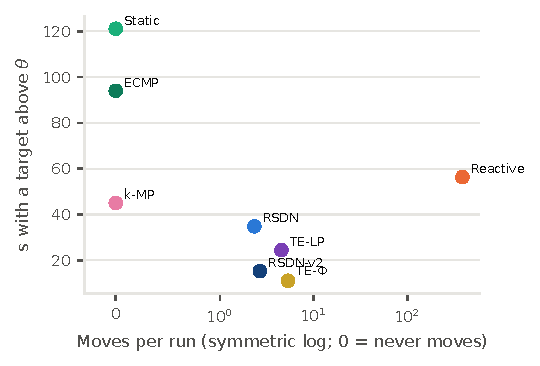
\includegraphics[width=\columnwidth]{figures/tradeoff}
\caption{Disruption (moves per run, log) against seconds a target is above $\theta$; means over all
attack scenarios, topologies and seeds (simulation).}\label{fig:tradeoff}
\end{figure}

\paragraph{WAN topologies, sustained and adversarial attacks (S6--S10)}
Fig.~\ref{fig:wan_adversarial} extends S6, S7, S8 and S10 to the three WANs. In the 600\,s
overload S6, ResilientSDN cut the time above $\theta$ from 600\,s (static) to 6\,s on the
fat-tree, 46\,s on G\'EANT, 65\,s on NSFNET and 204\,s on Internet2, and v2 to 6--26\,s on all
four; loss of the victim flows fell from about 9--10\,\% to 0.1\,\%. The Internet2 value
reproduces, in simulation, the hold that the emulation showed for Internet2 S11
(Sec.~\ref{sec:formulation}): with the sum drift, a 7--13-hop detour scores worse than the
congested one-hop link, so the deadband keeps the flow. The pulse attack S7 evades the trend
detector on every topology (ResilientSDN = static, 32\,s); the timed attack S8 is relieved within the
detection delay (6\,s). Under S10 (one of S7--S9 against randomised $N$ and cooldown) ResilientSDN
kept the target above $\theta$ for 8--25\,s against 30--33\,s for static routing; simple reactive was
lower on Internet2 and NSFNET, where S10 drew pulse runs, and v2 was at 8--15\,s.

\begin{figure*}[t]\centering
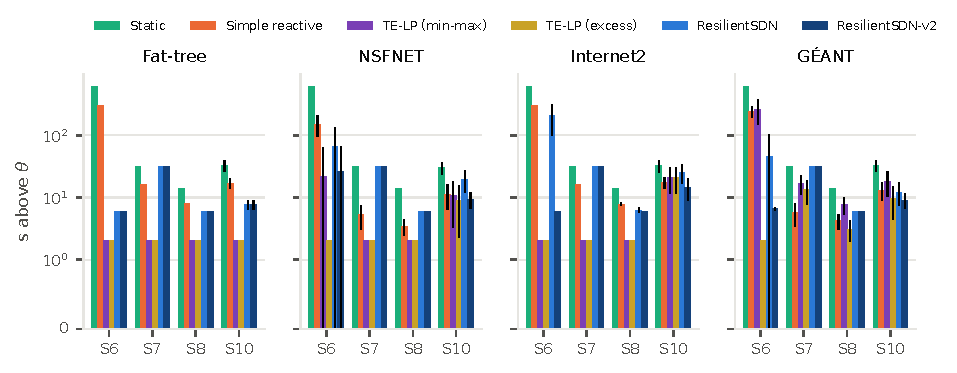
\includegraphics[width=\textwidth]{figures/wan_adversarial}
\caption{Seconds above $\theta$ for S6--S10 on all four topologies (simulation, mean and 95\,\% CI
over 30 seeds; symmetric-log axis).}\label{fig:wan_adversarial}
\end{figure*}

\paragraph{Closing the pulse loophole (v3)}
Table~\ref{tab:v3} adds the duty-cycle trigger (react when a link is above $\theta$ now and in at
least 3 of the last 6 polls) to ResilientSDN (+Duty) and to v2 (v3), over 13 scenarios, four
topologies and 30 seeds. It removes the pulse evasion of S7 on every topology (32 to 6\,s above
$\theta$) and lowers S10 from 16.2 to 13.6\,s (v2: 10.2 to 8.2\,s); averaged over all attacks, v3
keeps a target above $\theta$ for 11.8\,s, against 15.3\,s for v2 and 34.8\,s for ResilientSDN.
The cost is small: no move without an attack, neither in S1 nor under the legitimate bursts of SB
(where simple reactive rerouting made 14.8 moves per run and TE-$\Phi$ 2.4), unchanged secondary
congestion, and 0.1 more moves per run. In the paired tests (52 cells, Holm-corrected), v3 has
significantly less time above $\theta$ than ResilientSDN in 16 cells and more in none, and makes
significantly more moves in 8. The randomised sweep (Sec.~\ref{sec:sweep}) confirms the effect for
random pulse periods and duty cycles.
\IfFileExists{generated/tab_v3.tex}{\begin{table}[t]\centering\scriptsize
\caption{Duty-cycle trigger (simulation, 4 topologies $\times$ 30 seeds): +Duty adds it to the published ResilientSDN, v3 adds it to v2. False moves are reroutes when no attack is present.}
\label{tab:v3}
\begin{tabular}{lrrrr}
\toprule
 & RSDN & +Duty & RSDN-v2 & RSDN-v3\\
\midrule
False moves, S1 & 0.00 & 0.00 & 0.00 & 0.00\\
False moves, bursts (SB) & 0.00 & 0.00 & 0.00 & 0.00\\
s above $\theta$, S7 pulse & 32.0 & 6.0 & 32.0 & 6.0\\
s above $\theta$, S10 & 16.2 & 13.6 & 10.2 & 8.2\\
s above $\theta$, all attacks & 34.8 & 31.6 & 15.3 & 11.8\\
Victim loss \%, all attacks & 0.72 & 0.68 & 0.55 & 0.48\\
Secondary congestion & 0.05 & 0.05 & 0.35 & 0.36\\
Moves per run, all attacks & 2.3 & 2.4 & 2.7 & 2.8\\
\bottomrule
\end{tabular}
\end{table}}{}

\IfFileExists{generated/tab_wan_ext.tex}{\begin{table}[t]\centering\scriptsize
\caption{Mininet emulation of the scenarios added on the WANs in revision 4 (means over $n$ runs): legitimate loss (\%), seconds the target was above $\theta$, reroutes.}
\label{tab:wan_ext}
\setlength{\tabcolsep}{2.5pt}
\begin{tabular}{llrccc}
\toprule
Topology & Scen. & $n$ & Static & Reactive & RSDN\\
\midrule
NSFNET & S7 & 5 & 0.73 | 18 | 0.0 & 0.01 | 2 | 6.0 & 0.02 | 16 | 0.0\\
NSFNET & S8 & 5 & 0.64 | 12 | 0.0 & 0.00 | 6 | 12.6 & 0.06 | 6 | 1.2\\
NSFNET & S10 & 5 & 3.98 | 25 | 0.0 & 21.10 | 15 | 138.0 & 2.65 | 17 | 1.8\\
Internet2 & S7 & 5 & 0.00 | 27 | 0.0 & 0.43 | 12 | 46.4 & 0.00 | 27 | 0.0\\
Internet2 & S8 & 5 & 0.00 | 12 | 0.0 & 0.00 | 8 | 24.2 & 0.00 | 7 | 0.8\\
Internet2 & S10 & 5 & 0.92 | 34 | 0.0 & 19.30 | 20 | 213.2 & 1.31 | 32 | 2.2\\
G\'EANT & S7 & 3 & 0.00 | 26 | 0.0 & 0.00 | 2 | 5.3 & 0.00 | 26 | 0.0\\
\bottomrule
\end{tabular}
\end{table}}{}
\paragraph{WAN emulation of S6--S10}
% WAN-EMULATION-PARAGRAPH (filled in from generated/wan_ext_summary.csv when the campaign ends)

\paragraph{Multiple attacked links (S12, S13)}
With two or three simultaneously attacked links (Fig.~\ref{fig:multilink}), ResilientSDN's
single-link behaviour carries over on the fat-tree (12\,s for S12, 27\,s for S13) but not on the
WANs: 98 and 109\,s of 120\,s on G\'EANT, 40 and 83\,s on Internet2 (the long-detour hold again) and
25 and 109\,s on NSFNET. On NSFNET S13 no system kept the targets below $\theta$ for long (v2 51\,s,
TE-$\Phi$ 85\,s): three disjoint attacks on a 15-link network leave few detours with enough capacity. ResilientSDN-v2 reduced the time above $\theta$ to 6--16\,s on
fat-tree, Internet2 and G\'EANT and to 51\,s on NSFNET S13, and victim loss on G\'EANT from 5.3\,\%
to 2.0\,\% (S12). In S13, v2 is lower than TE-$\Phi$ (22\,s against 40\,s, mean over topologies),
whose six candidate paths per flow do not include the detours v2 finds within the hop limit.

\begin{figure*}[t]\centering
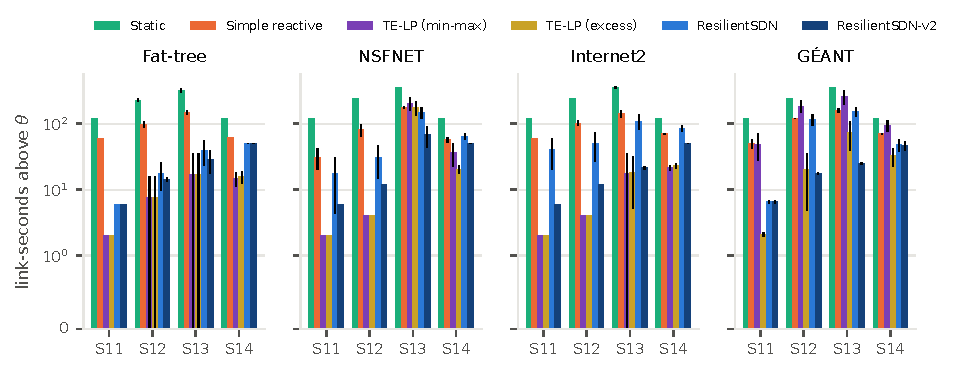
\includegraphics[width=\textwidth]{figures/multilink}
\caption{Link-seconds above $\theta$ summed over all targets: one target (S11), two (S12), three
(S13), and the adaptive attacker (S14). Simulation, 30 seeds.}\label{fig:multilink}
\end{figure*}

\paragraph{Adaptive rolling attacker (S14)}
When the attacker re-aims every 10\,s at the link the victims now share, every reactive defence
loses part of its advantage: ResilientSDN kept a target above $\theta$ for 48--86\,s of 120\,s
(static: 120\,s; v2: 47--50\,s), making 8--12 moves per run as it followed the attacker. TE-$\Phi$
did better on all four topologies (16--33\,s) and min-max TE-LP on three (it fails on G\'EANT,
94\,s, for the reason given above). $k$-path multipath was the most robust defence on fat-tree and
NSFNET (0--4\,s), since a fixed bot budget spread over three paths cannot push one link over
$\theta$, but not on Internet2 and G\'EANT (56--84\,s). Victim loss was 2--4\,\% for ResilientSDN,
9--10\,\% for static routing and below 1\,\% for TE-$\Phi$.

\paragraph{Presaturation (S9) and the cost of the fallback}
Simple reactive rerouting and $k$-path multipath both put traffic onto the pre-filled paths and lost
38--46\,\% and 10--33\,\% of the victim traffic on the WANs; the capacity filter kept ResilientSDN
at 0\,\%. The fallback of v2 halves the time above $\theta$ in S9 (27\,s to 12\,s), but by design
it may load a path above $\theta$: secondary congestion rises from 0.04 to 2.4 links per run on
average and to 6.7 on Internet2.
Table~\ref{tab:ablation_v2} separates the three v2 extensions: the bottleneck drift alone gives
most of the gain in S11--S14, the fallback acts only where no path passes the filter (S9, S13)
and is the one that causes the secondary congestion, and the severity order alone changes
nothing measurable. An operator who values ``no collateral congestion'' over relief time should
keep the fallback off; Proposition~\ref{prop:monotone} then holds.

\begin{table}[t]\centering\scriptsize
\caption{ResilientSDN-v2 ablation (simulation, mean over 4 topologies $\times$ 30 seeds): link-seconds above $\theta$ / victim loss (\%) / secondary congestion. Each extension alone, then all three (v2).}
\label{tab:ablation_v2}
\setlength{\tabcolsep}{2pt}
\begin{tabular}{lccccc}
\toprule
Scen. & RSDN & +Severity & +Fallback & +Bottleneck & RSDN-v2\\
\midrule
S9 & 27.2/0.00/0.04 & 27.2/0.00/0.03 & 12.4/0.00/2.22 & 24.8/0.00/0.03 & 12.5/0.00/2.36\\
S11 & 17.6/0.47/0.00 & 17.6/0.47/0.00 & 17.6/0.47/0.00 & 6.2/0.47/0.00 & 6.2/0.47/0.00\\
S12 & 53.8/1.92/0.02 & 51.9/2.03/0.02 & 55.6/1.56/0.07 & 15.8/1.06/0.03 & 13.9/1.05/0.08\\
S13 & 112.3/2.47/0.03 & 114.0/2.48/0.03 & 85.3/1.69/0.55 & 56.4/1.20/0.04 & 35.5/1.18/0.47\\
S14 & 62.2/2.96/0.43 & 62.2/2.96/0.43 & 62.0/2.99/0.48 & 50.7/3.15/0.10 & 49.2/3.21/0.12\\
\bottomrule
\end{tabular}
\end{table}

\paragraph{TCP goodput and flow-completion time}
With the legitimate flows as TCP transfers of 5\,MB (ideal FCT 2.0\,s), static routing raised the
mean FCT to 7.9--17\,s under overload (S6, S11--S13) and simple reactive rerouting to 4.5--16\,s,
partly because its oscillation moves the transfers between congested paths. ResilientSDN and v2
kept the mean FCT at 2.0--3.3\,s in every cell (Table~\ref{tab:sim_fct}, Fig.~\ref{fig:tcp_fct});
TE-$\Phi$ was closest to ideal (2.0--2.4\,s). The adaptive attacker (S14) is the scenario where
ResilientSDN's FCT rises most (2.6--3.3\,s), because victims are hit again after each move.
The fluid TCP model assumes that a TCP flow keeps at least 5\,\% of a saturated link. Re-running
S6 and S11--S14 with this floor at 0 and at 10\,\% (\floorCells{} topology--scenario cells, 30
seeds) changed the mean FCT of ResilientSDN, v2 and TE-$\Phi$ by at most 6\,\% and left the median
cell unchanged; static routing and simple reactive rerouting are more sensitive (up to
\floorMaxRel\,\%). The ranking changed in \floorFlips{} cells, but only between systems within
0.1\,s of each other (TE-$\Phi$, ResilientSDN, v2) or between static and simple reactive; the two
groups never swapped, so the TCP conclusions do not depend on the floor.

\begin{table*}[t]\centering\scriptsize
\caption{Simulation, TCP legitimate traffic: mean flow-completion time of 5\,MB transfers that start during the attack, s (mean $\pm$ 95\% CI, 30 seeds; ideal 2.0\,s).}\label{tab:sim_fct}
\setlength{\tabcolsep}{3pt}
\begin{tabular}{llrrrrrrrr}
\toprule
Topology & Scen. & Static & ECMP & k-MP & Reactive & TE-LP & TE-$\Phi$ & RSDN & RSDN-v2\\
\midrule
Fat-tree & S3 & 2.6$\pm$0.0 & 2.0$\pm$0.0 & \textbf{2.0} & 2.3$\pm$0.1 & \textbf{2.0} & \textbf{2.0} & 2.0 & 2.0\\
 & S6 & 7.9$\pm$0.0 & \textbf{2.0} & \textbf{2.0} & 6.5$\pm$0.9 & \textbf{2.0} & \textbf{2.0} & 2.0$\pm$0.0 & 2.0$\pm$0.0\\
 & S9 & 2.6$\pm$0.0 & \textbf{2.0} & \textbf{2.0} & 2.5$\pm$0.1 & 2.0$\pm$0.0 & 2.0$\pm$0.0 & 2.1$\pm$0.0 & 2.1$\pm$0.0\\
 & S11 & 7.9$\pm$0.0 & 2.0$\pm$0.1 & \textbf{2.0} & 6.6$\pm$0.9 & \textbf{2.0} & \textbf{2.0} & 2.0 & 2.0\\
 & S12 & 11.1$\pm$1.9 & 2.5$\pm$0.2 & 2.1$\pm$0.1 & 6.5$\pm$0.9 & 2.0$\pm$0.0 & \textbf{2.0$\pm$0.0} & 2.1$\pm$0.1 & 2.1$\pm$0.1\\
 & S13 & 12.5$\pm$2.1 & 2.4$\pm$0.2 & 2.2$\pm$0.1 & 7.1$\pm$1.1 & 2.0$\pm$0.0 & \textbf{2.0$\pm$0.0} & 2.2$\pm$0.1 & 2.1$\pm$0.1\\
 & S14 & 8.1$\pm$0.4 & 3.2$\pm$0.7 & \textbf{2.0} & 5.3$\pm$0.9 & 2.1$\pm$0.0 & 2.1$\pm$0.0 & 2.8$\pm$0.0 & 2.9$\pm$0.0\\
\midrule
NSFNET & S3 & 2.6$\pm$0.0 & 2.6$\pm$0.0 & \textbf{2.0} & 2.3$\pm$0.2 & \textbf{2.0} & 2.0$\pm$0.0 & 2.1$\pm$0.0 & 2.0\\
 & S6 & 7.9$\pm$0.0 & 7.9$\pm$0.0 & \textbf{2.0$\pm$0.1} & 4.9$\pm$1.8 & 2.1$\pm$0.1 & 2.0$\pm$0.1 & 2.0$\pm$0.1 & 2.0$\pm$0.1\\
 & S9 & 2.6$\pm$0.0 & 2.6$\pm$0.0 & 2.9$\pm$0.2 & 11.4$\pm$1.4 & 2.2$\pm$0.1 & 2.2$\pm$0.1 & 2.5$\pm$0.1 & \textbf{2.1$\pm$0.0}\\
 & S11 & 7.9$\pm$0.0 & 7.9$\pm$0.0 & \textbf{2.0} & 4.5$\pm$1.6 & \textbf{2.0} & \textbf{2.0} & 2.0$\pm$0.0 & 2.0$\pm$0.0\\
 & S12 & 7.9$\pm$0.0 & 7.9$\pm$0.0 & 2.0$\pm$0.0 & 4.6$\pm$0.8 & \textbf{2.0} & \textbf{2.0} & 2.1$\pm$0.0 & 2.0\\
 & S13 & 7.9$\pm$0.2 & 7.9$\pm$0.2 & 2.8$\pm$0.1 & 7.3$\pm$1.5 & 2.2$\pm$0.0 & 2.3$\pm$0.1 & 2.4$\pm$0.2 & \textbf{2.1$\pm$0.0}\\
 & S14 & 7.9$\pm$0.0 & 7.9$\pm$0.0 & \textbf{2.0$\pm$0.0} & 6.3$\pm$1.6 & 2.1$\pm$0.0 & 2.2$\pm$0.0 & 2.7$\pm$0.4 & 2.8$\pm$0.0\\
\midrule
Internet2 & S3 & 2.6$\pm$0.0 & 2.6$\pm$0.0 & 2.1$\pm$0.1 & 2.8$\pm$0.1 & \textbf{2.0} & \textbf{2.0} & 2.1$\pm$0.1 & 2.0\\
 & S6 & 7.9$\pm$0.0 & 7.9$\pm$0.0 & 2.2$\pm$0.2 & 10.8$\pm$1.5 & \textbf{2.0} & \textbf{2.0} & 2.2$\pm$0.1 & 2.0$\pm$0.0\\
 & S9 & 2.6$\pm$0.0 & 2.6$\pm$0.0 & 4.6$\pm$0.6 & 11.2$\pm$1.5 & 2.6$\pm$0.1 & 2.7$\pm$0.1 & 2.7$\pm$0.1 & \textbf{2.1$\pm$0.0}\\
 & S11 & 7.9$\pm$0.0 & 7.9$\pm$0.0 & 2.1$\pm$0.1 & 9.5$\pm$1.1 & \textbf{2.0} & \textbf{2.0} & 2.1$\pm$0.1 & 2.0$\pm$0.0\\
 & S12 & 8.0$\pm$0.2 & 8.0$\pm$0.2 & 2.1$\pm$0.1 & 6.1$\pm$1.1 & \textbf{2.0} & \textbf{2.0} & 2.1$\pm$0.1 & 2.0$\pm$0.0\\
 & S13 & 10.6$\pm$0.8 & 10.6$\pm$0.8 & 2.7$\pm$0.2 & 8.0$\pm$1.5 & \textbf{2.0$\pm$0.0} & 2.0$\pm$0.1 & 2.4$\pm$0.2 & 2.2$\pm$0.1\\
 & S14 & 7.9$\pm$0.0 & 7.9$\pm$0.0 & \textbf{2.1$\pm$0.1} & 9.3$\pm$1.3 & 2.2$\pm$0.2 & 2.1$\pm$0.0 & 3.3$\pm$0.5 & 2.9$\pm$0.1\\
\midrule
G\'EANT & S3 & 2.8$\pm$0.1 & 2.8$\pm$0.1 & 2.1$\pm$0.1 & 2.8$\pm$0.3 & 2.4$\pm$0.2 & 2.1$\pm$0.1 & 2.1$\pm$0.1 & \textbf{2.0$\pm$0.0}\\
 & S6 & 10.3$\pm$1.4 & 10.3$\pm$1.4 & 2.7$\pm$0.4 & 6.5$\pm$1.9 & 5.9$\pm$2.0 & 2.0$\pm$0.0 & 2.0$\pm$0.1 & \textbf{2.0$\pm$0.0}\\
 & S9 & 2.7$\pm$0.1 & 2.7$\pm$0.1 & 9.2$\pm$1.7 & 11.9$\pm$1.4 & 2.4$\pm$0.1 & 2.1$\pm$0.1 & 2.1$\pm$0.1 & \textbf{2.1$\pm$0.0}\\
 & S11 & 10.1$\pm$1.2 & 10.1$\pm$1.2 & 2.6$\pm$0.3 & 6.9$\pm$2.1 & 5.9$\pm$2.0 & \textbf{2.0$\pm$0.0} & 2.0$\pm$0.0 & 2.0$\pm$0.0\\
 & S12 & 17.0$\pm$2.2 & 17.0$\pm$2.2 & 4.3$\pm$0.5 & 16.3$\pm$2.5 & 13.4$\pm$3.2 & \textbf{2.0$\pm$0.1} & 2.8$\pm$0.4 & 2.2$\pm$0.1\\
 & S13 & 12.7$\pm$1.3 & 12.7$\pm$1.3 & 3.5$\pm$0.3 & 8.1$\pm$1.3 & 9.4$\pm$2.4 & \textbf{2.1$\pm$0.1} & 2.4$\pm$0.2 & 2.2$\pm$0.1\\
 & S14 & 9.4$\pm$1.1 & 9.4$\pm$1.1 & 3.7$\pm$0.9 & 8.7$\pm$1.5 & 6.7$\pm$1.5 & \textbf{2.4$\pm$0.3} & 2.6$\pm$0.8 & 2.4$\pm$0.3\\
\bottomrule
\end{tabular}
\end{table*}
\begin{figure*}[t]\centering
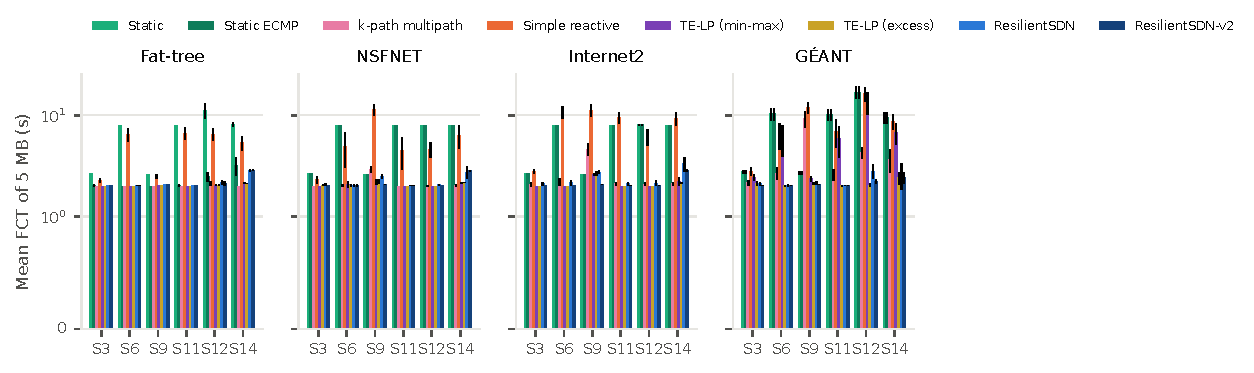
\includegraphics[width=\textwidth]{figures/tcp_fct}
\caption{Mean flow-completion time of the victims' 5\,MB TCP transfers (simulation, 30 seeds).}
\label{fig:tcp_fct}
\end{figure*}

\paragraph{ECMP against an ECMP-aware attacker}
With targets planned from static routes, ECMP and $k$-path multipath avoid the fat-tree attacks
altogether (Table~\ref{tab:sim_time}), which flatters them: the attack never reaches the link they
use. When the attacker picks host pairs that cross the target under both static and ECMP routing
(as Crossfire's route mapping would), ECMP is identical to static routing on every topology
(60 and 120\,s, Table~\ref{tab:sim_ecmp}), while ResilientSDN's results are similar to those with
the default attacker (the host pairs differ, so the values are not identical).

\begin{table*}[t]\centering\scriptsize
\caption{Simulation with an ECMP-aware attacker (attack pairs cross the target under both static and ECMP routing): seconds above $\theta$.}\label{tab:sim_ecmp}
\setlength{\tabcolsep}{3pt}
\begin{tabular}{llrrrrrrr}
\toprule
Topology & Scen. & Static & ECMP & k-MP & Reactive & TE-LP & RSDN & RSDN-v2\\
\midrule
Fat-tree & S3 & 60 & 60 & \textbf{0} & 26$\pm$4 & 2 & 6 & 6\\
 & S5 & 60 & 60 & \textbf{0} & 30 & 2 & 6 & 6\\
 & S9 & 54 & 54 & \textbf{0} & 27$\pm$2 & 2 & 6 & 6\\
 & S11 & 120 & 120 & \textbf{0} & 60 & 2 & 6 & 6\\
\midrule
NSFNET & S3 & 60 & 60 & \textbf{0} & 15$\pm$5 & 2 & 6 & 6\\
 & S5 & 60 & 60 & \textbf{0} & 9$\pm$4 & 2 & 6 & 6\\
 & S9 & 54 & 54 & 60$\pm$1 & 29$\pm$0 & 28$\pm$10 & 40$\pm$8 & \textbf{10$\pm$4}\\
 & S11 & 120 & 120 & \textbf{0} & 31$\pm$11 & 2 & 17$\pm$13 & 6\\
\midrule
Internet2 & S3 & 60 & 60 & 16$\pm$10 & 28$\pm$3 & \textbf{2} & 11$\pm$6 & 6\\
 & S5 & 60 & 60 & \textbf{0} & 30 & 2 & 6 & 6\\
 & S9 & 54 & 54 & 57$\pm$1 & 29$\pm$3 & 52$\pm$4 & 52$\pm$3 & \textbf{27$\pm$8}\\
 & S11 & 120 & 120 & 56$\pm$23 & 60 & \textbf{2} & 40$\pm$20 & 6\\
\midrule
G\'EANT & S3 & 60 & 60 & 34$\pm$11 & 26$\pm$4 & 16$\pm$9 & 8$\pm$4 & \textbf{6}\\
 & S5 & 60 & 60 & 10$\pm$8 & 13$\pm$5 & 25$\pm$11 & \textbf{6} & \textbf{6}\\
 & S9 & 54 & 54 & 59$\pm$1 & 29$\pm$0 & 26$\pm$10 & 11$\pm$5 & \textbf{7$\pm$2}\\
 & S11 & 120 & 120 & 72$\pm$22 & 46$\pm$9 & 49$\pm$22 & \textbf{6} & \textbf{6}\\
\bottomrule
\end{tabular}
\end{table*}

% Revision 4 -- generalisation over the problem space (answers "the considered scenario is too simple").
% Numbers: paper_rev4/generated/{tab_sweep,tab_sweep_pattern}.tex, sweep_macros.tex, sweep_paired.csv,
% sweep_defendable.csv, sweep_family.csv; data results/sweep/*.csv (sim/sweep.py, sim/generic.py).
\subsection{Generalisation: a randomised sweep over the problem space}\label{sec:sweep}

S1--S14 are single points of the scenario space of Sec.~\ref{sec:formulation}. To test whether the
conclusions drawn from them carry over, we drew 2{,}000 instances at random from the ranges of
Table~\ref{tab:scenario_space} (\texttt{sim/generic.py}): the eight real topologies or a Waxman or
Barab\'asi--Albert graph of 15--40 nodes with uniform or mixed (10/40/100\,Mbps) capacities; a
gravity-model demand of 10--60 flows scaled so that static routing loads the busiest link to
U[0.2,\,0.6]; one to three attacked links, each with one to five bots; an attack intensity $\alpha$
(the targets' offered load over capacity) drawn from U[0.9,\,1.6]; and one of four behaviours ---
constant, pulsing (period 4 or 8\,s, duty $\tfrac13$, $\tfrac12$ or $\tfrac23$), timed bursts, or
rolling re-targeting at the link the victims share under the current routing. 55 instances, all
Waxman graphs, had no attackable link (every fastest link was a bridge or crossed by no host pair) and
were dropped; the remaining \sweepN{} instances (11--50 nodes, 14--99 links) were each run with seven
systems, \sweepRuns{} runs in total. All systems see the same instance (it is seeded by its id) and the
same candidate-path limit (the 20 lowest-latency paths within the hop limit). For every instance we
also solved (\ref{eq:phistar}), which gives $\Phi^\star$, defendability and the remaining excess of each
system. Under the rolling attack the demand depends on the routing, so $\Phi^\star$ is solved for each
system's own demand; when a system's reroutes provoke an attack whose $\Phi^\star$ is already at least
$\Phi_{\mathrm{static}}$ (40--84 rolling instances per system), the ratio is undefined, and we count the
instance as infinitely bad if the system's $\Phi$ exceeds $\Phi_{\mathrm{static}}$ and as 1 otherwise,
rather than dropping it.

\paragraph{Defendability}
\sweepDefend\,\% of the instances are defendable ($\Phi^\star=0$). As Proposition~\ref{prop:cut}
predicts, the share falls with the attack intensity and the number of targets: from 91\,\% for one
target and $\alpha\le1.1$ to 23\,\% for three targets and $\alpha>1.3$
(\texttt{sweep\_defendable.csv}). Sparse Waxman graphs are defendable less often (42\,\%) than
Barab\'asi--Albert graphs (68\,\%) and the real topologies (64\,\%), since they have fewer disjoint
detours. In the remaining 39\,\% no controller can keep every link below $\theta$, and the right
question is how close to $\Phi^\star$ a system gets, which the remaining excess measures.

\IfFileExists{generated/tab_sweep.tex}{\begin{table}[t]\centering\scriptsize
\caption{Randomised sweep over the problem space (1945 instances, Sec.~\ref{sec:sweep}). Remaining excess: $(\Phi-\Phi^\star)/(\Phi_{\mathrm{static}}-\Phi^\star)$, 0 = optimal, 1 = no better than static routing (median [IQR]); $>$static: share of instances with a remaining excess above 1. Relieved: share of defendable instances ($\Phi^\star=0$) in which no target stayed above $\theta$ for more than 10\,s. Victim loss and moves (flow reroutes) are means over all instances.}
\label{tab:sweep}
\setlength{\tabcolsep}{3pt}
\begin{tabular}{lrrrrr}
\toprule
System & remaining excess & $>$static & relieved & victim loss \% & moves\\
\midrule
Static & 1.00 [1.00, 1.00] & 0\% & 0\% & 16.00 & 0.0\\
k-MP & 0.49 [0.11, 4.39] & 32\% & 51\% & 9.67 & 0.0\\
Reactive & 1.44 [0.95, 4.75] & 71\% & 30\% & 18.43 & 359.3\\
TE-$\Phi$ & 0.09 [0.03, 0.13] & 3\% & 81\% & 4.17 & 10.4\\
RSDN & 0.70 [0.38, 0.99] & 8\% & 26\% & 7.34 & 6.8\\
RSDN-v2 & 0.52 [0.30, 0.98] & 9\% & 47\% & 6.83 & 8.0\\
RSDN-v3 & 0.40 [0.20, 0.78] & 9\% & 63\% & 5.61 & 8.9\\
\bottomrule
\end{tabular}
\end{table}}{}

\paragraph{Overall ranking}
Table~\ref{tab:sweep} and Fig.~\ref{fig:sweep_cdf} rank the systems over the whole space. The ordering
of the hand-made scenarios largely carries over, with one exception: $k$-MP, behind ResilientSDN in
S1--S14 (45 against 35\,s above $\theta$), is ahead of it here. TE-$\Phi$ comes closest to the optimum (median
remaining excess \sweepGaptelpexcess), followed by ResilientSDN-v3 (\sweepGapresilientsdnvThree),
$k$-MP (\sweepGapmpksp), v2 (\sweepGapresilientsdnvTwo), ResilientSDN (\sweepGapresilientsdn) and
simple reactive rerouting (\sweepGapsimplereactive, worse than static routing in 71\,\% of the
instances). $k$-MP and v2 have similar medians but different distributions: static three-way
splitting is worse than not reacting in 32\,\% of the instances (upper quartile 4.39), spread evenly
over all attack patterns, while the ResilientSDN variants are worse than static routing in 8--9\,\%,
almost all of them rolling attacks (below).
Paired over instances (Wilcoxon, Holm-corrected over the twelve comparisons with ResilientSDN), v3
has lower $\Phi$ than ResilientSDN in 1{,}277 instances, equal in 443 and higher in 225
($p<10^{-100}$, rank-biserial $-0.69$), and lowers the mean victim loss from 7.34 to 5.61\,\% (95\,\%
CI of the difference $[-1.99,-1.47]$ points); TE-$\Phi$ has lower $\Phi$ in 1{,}894 of the
1{,}945 instances. The remaining excess is a relative measure; in absolute terms, means are dominated
by a few instances with very large excess, which is why the table reports medians.

\begin{figure}[t]\centering
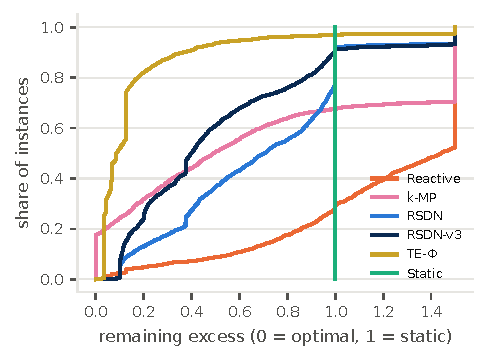
\includegraphics[width=\columnwidth]{figures/sweep_cdf}
\caption{Distribution of the remaining excess over the \sweepN{} sweep instances (0 = instance
optimum $\Phi^\star$, 1 = static routing; clipped at 1.5).}\label{fig:sweep_cdf}
\end{figure}

\IfFileExists{generated/tab_sweep_pattern.tex}{\begin{table}[t]\centering\scriptsize
\caption{Sweep by attack pattern: median remaining excess / share of defendable instances relieved (definitions as in Table~\ref{tab:sweep}). Instances per pattern: constant 519, timed 452, pulse 482, rolling 492.}
\label{tab:sweep_pattern}
\setlength{\tabcolsep}{3pt}
\begin{tabular}{lrrrr}
\toprule
System & constant & timed & pulse & rolling\\
\midrule
k-MP & 0.45 / 49\% & 0.45 / 59\% & 0.50 / 49\% & 0.54 / 47\%\\
Reactive & 1.55 / 8\% & 1.45 / 92\% & 1.38 / 12\% & 1.39 / 3\%\\
TE-$\Phi$ & 0.03 / 89\% & 0.13 / 88\% & 0.07 / 87\% & 0.13 / 51\%\\
RSDN & 0.39 / 42\% & 0.65 / 40\% & 1.00 / 6\% & 0.67 / 8\%\\
RSDN-v2 & 0.13 / 80\% & 0.46 / 69\% & 1.00 / 12\% & 0.56 / 8\%\\
RSDN-v3 & 0.13 / 80\% & 0.46 / 69\% & 0.27 / 69\% & 0.52 / 9\%\\
\bottomrule
\end{tabular}
\end{table}}{}

\paragraph{Where the hand-made conclusions do and do not generalise}
Fig.~\ref{fig:sweep_factors} and Table~\ref{tab:sweep_pattern} break the results down by factor.
\emph{(i) Pulsing attacks.} Over 482 pulsing instances with random periods and duty cycles,
ResilientSDN and v2 have a median remaining excess of 1.00 and relieve only 6 and 12\,\% of the
defendable ones: the trend detector's deadband evasion of S7 and Proposition~\ref{prop:evasion} is
not an artefact of one period, but holds over the sampled range. The duty-cycle trigger of v3 closes
most of it (0.27, 69\,\% relieved), and is equal to v2 on constant and timed attacks.
\emph{(ii) Rolling attacks} are the hardest case for every system: even TE-$\Phi$, which re-optimises
every interval, relieves 51\,\% of the defendable instances, and the reactive systems 3--9\,\%.
They are also the only case in which ResilientSDN does worse than not reacting: all 151 instances in
which its $\Phi$ exceeds that of static routing (31\,\% of the 492 rolling instances) are rolling
attacks; TE-$\Phi$ is worse than static routing in 11\,\% of them. The attacker re-aims at the link
the rerouted victims now share, so each reroute moves the congestion instead of removing it, while
static routing gives it no reason to move; the ten largest such losses are on G\'EANT (4), Arnes (5)
and one Waxman graph. Because of these instances the \emph{mean} $\Phi$ of ResilientSDN over the
whole sweep (134.5) exceeds that of static routing (119.8); without the rolling instances it is 40.3
against 60.0. Proposition~\ref{prop:monotone} does not contradict this: it holds for the measured
rates of one interval, and a routing-aware attacker changes the rates in the next.
\emph{(iii) Topology.} All systems are further from the optimum on sparse Waxman graphs (v3: 0.58
against 0.38 on the real topologies). On the real topologies, $k$-MP (0.34) is slightly ahead of v3
(0.38); on random graphs, with mixed capacities and less path diversity, it falls behind every
ResilientSDN variant. \emph{(iv) Intensity and number of targets.} TE-$\Phi$ is first and simple
reactive last in every $\alpha$ and target-count bin of Fig.~\ref{fig:sweep_factors}, and v3 is ahead
of v2 and v2 of ResilientSDN in every bin. $k$-MP is second for $\alpha\le1.1$ and for one target, but
falls behind v3 as the attack grows (median 0.29 to 0.58 over the $\alpha$ bins, against 0.34 to 0.48
for v3); it is level with v2 for $\alpha>1.3$ and behind it for three targets (0.62 against 0.54).

\begin{figure*}[t]\centering
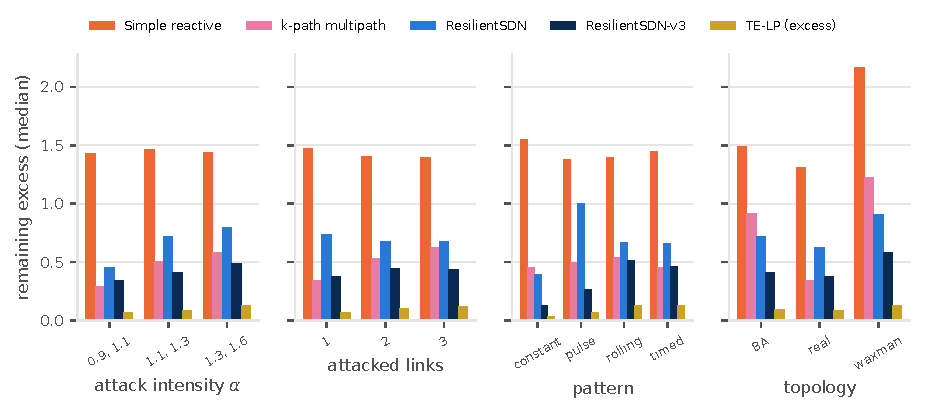
\includegraphics[width=\textwidth]{figures/sweep_factors}
\caption{Median remaining excess by attack intensity, number of attacked links, attack pattern and
topology family (\sweepN{} instances; 0 = instance optimum, 1 = static routing).}\label{fig:sweep_factors}
\end{figure*}

\paragraph{What the sweep does not cover}
The sweep runs in the flow-level simulator only, and $\Phi^\star$ is a relaxation: it splits flows
fractionally and knows the demand of each interval, so a remaining excess of 0 is a bound, not a
target an unsplittable reactive controller could reach. TE-$\Phi$ shares the fractional splitting and
the per-interval knowledge, which is why it is closest to $\Phi^\star$; it is an idealised reference,
not a deployable competitor (Sec.~\ref{sec:limits}).


\section{Related work additions}
% Revision 4 -- additions to Related Work (Sec. II) and a replacement Limitations section.

% ---- Related work: add after the existing SDN-defence paragraph --------------------------------
\paragraph{Link-flooding attacks}
Coremelt~\cite{studer2009coremelt} and Crossfire~\cite{kang2013crossfire} congest selected core
links with low-rate, legitimate-looking flows, and Crossfire's \emph{rolling} variant moves the
target as soon as routing reacts. CoDef~\cite{lee2013codef} reroutes and rate-controls with
collaborating ASes; SPIFFY~\cite{kang2016spiffy} temporarily increases bandwidth to tell
rate-adaptive (legitimate) from fixed-rate (bot) senders; Liaskos et al.~\cite{liaskos2016novel}
reroute to make attack flows identifiable. ResilientSDN does not try to identify attack flows; it
limits the damage they do within one domain, and our S14 scenario adopts the rolling attacker of
Crossfire.

\paragraph{Traffic engineering and multipath routing}
Offline TE optimises link weights for the expected demand~\cite{fortz2000ospf}; online TE such as
TeXCP~\cite{kandula2005texcp} balances load across pre-computed paths with stability guarantees, and
SDN WANs (B4~\cite{jain2013b4}, SWAN~\cite{hong2013swan}) solve LPs over tunnels with
congestion-free updates. Data-centre schemes spread load in the data plane: ECMP~\cite{rfc2992},
MPTCP~\cite{raiciu2011mptcp}, CONGA~\cite{alizadeh2014conga}. These systems target utilisation
under benign demand, split flows and assume demands are honest; ResilientSDN keeps flows
unsplit, changes as few rules as possible and uses a trend detector and hysteresis so that an
attacker cannot easily drive it into oscillation. Our TE-LP and $k$-MP baselines
(Sec.~\ref{sec:baselines}) represent these two families.

% ---- Limitations (replace the existing section) -------------------------------------------------
\section{Limitations and Threats to Validity}\label{sec:limits}
\begin{itemize}
\item \textbf{Two evaluation methods.} The S12--S14 scenarios, the TCP experiments, the 30-seed
  cells and the $k$-MP/TE-LP baselines come from the flow-level simulator, not from Mininet. The
  simulator runs the same decision code and agrees with the emulation on ranking
  (Sec.~\ref{sec:sim}), but it omits queueing, sub-second TCP dynamics and control-plane delay, so
  its absolute times and losses are not emulation results.
\item \textbf{TCP model.} TCP is a fluid max-min share with an assumed 5\,\% floor on saturated
  links; real TCP under a UDP flood may fare worse (timeouts) or better. Varying the floor between 0
  and 10\,\% changes the FCT of the rerouting systems by at most 6\,\% and does not reorder the two
  groups of systems (Sec.~\ref{sec:results}), but it is no substitute for packet-level TCP. FCT
  differences between systems are more reliable than FCT values.
\item \textbf{The LP baselines are idealised.} TE-LP and TE-$\Phi$ split flows fractionally, solve to optimality every
  interval and react on one poll; a deployable TE would round, rate-limit updates and pay
  select-group rule costs. Its results bound what any path-based TE could achieve with the same
  measurements; they are not a like-for-like comparison of deployability.
\item \textbf{Myopic, greedy control.} Algorithm~\ref{alg:rsdn} solves neither the horizon problem
  (\ref{eq:objective}) nor its single-interval version optimally; Proposition~\ref{prop:monotone}
  only guarantees monotone improvement for measured rates. The sum-drift score holds flows on
  congested links when only long detours exist (Internet2); ResilientSDN-v2 addresses this but has
  been evaluated in simulation only.
\item \textbf{Attacker model.} Attack targets are planned from static routes (S2--S13) or from the
  victims' observed routes (S14). An attacker that knows the controller's parameters can still
  evade the trend detector with pulses shorter than $N\tau$ (S7) and keep a link above $\theta$ up to
  two thirds of the time (Proposition~\ref{prop:evasion}); randomising $N$ (S10) only partly removes
  this. The duty-cycle trigger lowers the bound to one third but does not remove it, and it has been
  evaluated in simulation only. Against the routing-aware rolling attacker, rerouting can be worse
  than not reacting: in the sweep this happened in 31\,\% of the rolling instances for ResilientSDN
  and 11\,\% for TE-$\Phi$ (Sec.~\ref{sec:sweep}). A defence would need to stop moving traffic once
  the target follows it (e.g.\ by detecting re-targeting), which we have not implemented.
\item \textbf{Coverage of the scenario space.} The randomised sweep samples the ranges of
  Table~\ref{tab:scenario_space}, not every possible network or attacker: topologies up to 50
  nodes, one host per switch, constant-rate gravity demands, at most three targets and one rolling
  attacker, and a 60\,s attack. It runs in the simulator only, and its reference $\Phi^\star$ is a
  fractional, per-interval relaxation, so it bounds what any controller could achieve rather than
  what an unsplittable online controller can.
\item \textbf{Validation data and host load.} The simulator was validated against the summary
  table of a 1~October emulation campaign (54 points), not against the per-run data of the campaign
  reported in Sec.~V. Emulation is sensitive to host load: a first attempt at the WAN extension ran
  next to the simulation campaign and showed 5--10\,\% loss caused by CPU contention; those runs were
  discarded and all reported emulation runs were made on an otherwise idle host.
\item \textbf{Scale.} Emulated WANs have one host per PoP and capacities scaled to 100\,Mbps; five
  emulation runs per cell give wide intervals. The WAN emulation of S6 (600\,s attacks) has the
  number of completed runs given in Table~\ref{tab:wan_ext}.
\item \textbf{No identification of attack flows.} ResilientSDN moves the largest flows first and
  these are often attack flows; it limits congestion but does not stop the attack, and a
  sufficiently large botnet saturates every cut.
\end{itemize}


\bibliographystyle{IEEEtran}
\bibliography{references_rev4}
\end{document}
